\documentclass[12pt]{extreport}

\usepackage[top=1in,bottom=1.25in,left=1.5in,right=1in]{geometry}
\usepackage{array}
\usepackage{float}
\usepackage{amsfonts}
\usepackage{graphicx}
\usepackage{wrapfig}
\usepackage{setspace}
\usepackage{pgf}
\usepackage{tikz}
\usetikzlibrary{arrows,automata}
\usetikzlibrary{shapes.geometric,fit}
\usepackage{titlesec}
\usepackage{tocloft}
\usepackage{longtable}
\usepackage{lscape}
\usepackage[nottoc]{tocbibind}
\usepackage{fancyhdr}
\usepackage{inputenc}
\usepackage{enumitem}
\usepackage{titlesec}
\usepackage{fixltx2e}
\titleformat{\chapter}[display]
{\normalfont\huge\bfseries\centering}{\chaptertitlename\ \thechapter}{14pt}{\Huge}


\renewcommand{\cftaftertoctitle}{\hrulefill}

\renewcommand*\contentsname{CONTENTS}
\renewcommand*{\listfigurename}{LIST OF FIGURES}
\renewcommand*{\listtablename}{LIST OF TABLES}


\setlist[enumerate,1]{label={(\alph*)}}
\setlist[enumerate,2]{label={(\roman*)}}

\newcounter{parnum}
\newcommand{\N}{%
   \noindent\refstepcounter{parnum}%
    \makebox[\parindent][l]{\textbf{\arabic{parnum}.}}}
    
 \setlength{\parindent}{5em}
    
         
 \renewcommand{\arraystretch}{1.2}  
 
\newcolumntype{M}[1]{>{\centering\arraybackslash}m{#1}} 

\renewcommand{\cfttoctitlefont}{\hspace*{\fill}\Huge\bfseries}
\renewcommand{\cftaftertoctitle}{\hspace*{\fill}}
\renewcommand{\cftlottitlefont}{\hspace*{\fill}\Huge\bfseries}
\renewcommand{\cftafterlottitle}{\hspace*{\fill}}
\renewcommand{\cftloftitlefont}{\hspace*{\fill}\Huge\bfseries}
\renewcommand{\cftafterloftitle}{\hspace*{\fill}}


\begin{document}
\begin{titlepage}
\begin{titlepage}
\centering


%\end{document}

%\onehalfspacing
\textbf{A PROJECT REPORT ON}\\\vspace{1cm}\large\textbf{"Confidential log in to real user using Visual Cryptography and upload encrypted data on Database System using Steganography"}\\\vspace{1cm}

SUBMITTED TO THE SAVITRIBAI PHULE PUNE UNIVERSITY, PUNE
IN THE PARTIAL FULFILLMENT OF THE REQUIREMENTS 
FOR THE AWARD OF THE DEGREE 
\begin{center}

\vspace{1cm} OF\\\vspace{1cm}\textbf{BACHELOR OF ENGINEERING (COMPUTER ENGINEERING) }\\\vspace{1cm}BY\vspace{1cm}\\
{\small{MANOJ WAGHMARE} \hspace{22mm} {\small ROLL NO:13CO063}\\{SHUBHAM SHETYANAVAR} \hspace{13mm} {\small ROLL NO:13CO054 } \\{SHRENIK SHAH} \hspace{32mm} {\small ROLL NO:13CO051} \\{SAURABH GANDHI } \hspace{26.8mm} {\small ROLL NO:12CO039 }\\\vspace{1cm}}
\end{center}
\textbf{DEPARTMENT OF COMPUTER ENGINEERING}\\ 
\textbf{AISSMS COLLEGE OF ENGINEERING} \\
\begin{center}
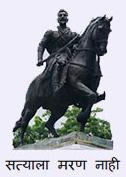
\includegraphics[scale=0.6]{logo.png}
\end{center}
Kennedy Road, Near R.T.O Office, Pune, Maharashtra 411001

2016-2017
\end{titlepage}

\end{titlepage}

\pagenumbering{roman}
\setcounter{page}{2}
%\usepackege{setspace}
%\documentclass[letterpaper,12pt]{article}

%\begin{document}
%\fancyput*(x,y){LR stuff }
%\thisfancyput*(x,y){LR stuff }
\noindent
\begin{wrapfigure}{l}{0.2\textwidth}
  \begin{flushleft}
    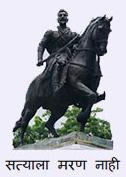
\includegraphics[width=2cm]{logo.png}
  \end{flushleft}
  \end{wrapfigure}
 
	
%\end{document}
\begin {center}
{\LARGE\bf CERTIFICATE}\\\vspace{1.4cm}
\large {This is to certify that the project report entitles}\\\vspace{0.7cm}

{\bf "Confidential log in to real user using Visual Cryptography and upload encrypted data on Database System using Steganography"}\\\vspace{0.7cm}

\large {Submitted by}\\\vspace{0.5cm}
{\small\bf{MANOJ WAGHMARE} \hspace{19mm} {\small ROLL NO:13CO063 }\\{SHUBHAM SHETYANAVAR} \hspace{5.5mm} {\small ROLL NO:13CO054 } \\{SHRENIK SHAH} \hspace{29mm} {\small ROLL NO:13CO050} \\{SAURABH GANDHI} \hspace{20.8mm} {\small ROLL NO:13CO018 }\\\vspace{1cm}}
\end{center}
\vspace{3mm} 

%\paragraph{}
%\begin{flushleft}
\noindent
is a bonafide work carried out by them under the supervision of \textbf{Prof A.S. Deokar} and it is approved for the partial fulfillment of the requirement of Savitribai Phule Pune University Pune for the award of the degree of Bachelor of Engineering (Computer Engineering) \\

\noindent
This project work has not been earlier submitted to any other Institute or University for the award of any degree or diploma.

%\end{flushleft}


\vspace{1cm}
\begin{flushleft}


\begin{tabular}{c c } 
\bf Prof A.S.Deokar &\hspace{1.5cm}\bf Dr D.P.Gaikwad \\
\bf Guide&\hspace{1.8cm}\bf Head,\\
\bf Department of Computer Engineering &\hspace{0.75cm} \bf Department of Computer Engineering 
 
\end{tabular}
\end{flushleft}\\
\vspace{1cm}
\begin{center}
\hspace{10mm}\bf{Dr S.P.Danao\\\hspace{5mm}Principal\\\hspace{5mm}AISSMS College of Engineering}
\end{center}
\begin{flushleft}
Place : Pune\\
Date  :  
\end{flushleft}

\pagenumbering{gobble}
\chapter*{\Huge\textbf{ACKNOWLEDGEMENT}}

 We would like to extend my sincere gratitude and thanks to my guide \textbf{Prof A.S. Deokar}, for his invaluable guidance and for giving us useful inputs and encouragement time and again, which inspired us to work harder.  Due to his forethought, appreciation of the work involved and continuous imparting of useful tips, this report has been successfully completed.\\

\noindent
We are extremely grateful to \textbf{Dr D.P.Gaikwad}, Head of the Department of Computer Engineering, for his  encouragement during the course of the project work.\\   

\noindent
We also extend our heartfelt gratitude to the staff of Computer Engineering Department for their cooperation and support. \\

\noindent
We also take this opportunity to thank all our classmates,friends and all those who have directly or indirectly provided their overwhelming support during  our project work and the development of this report.\\






\vspace{0.5in}
\begin{tabular}{ll}
 & \hspace{3.5in} \bf Manoj Waghmare\\
 & \hspace{3.5in} \bf Shubham Shetyanavar\\
 & \hspace{3.5in} \bf Saurabh Gandhi\\
 & \hspace{3.5in} \bf Shrenik Shah\\
\end{tabular}
\pagenumbering{gobble}

\chapter*{\Huge\textbf{ABSTRACT}}

\hspace*{5em}Data is an important asset for any individual or organization and must be protected from intruders or hackers. The need to hide data from hackers has existed since ancient times, and nowadays, there are developments in digital media, such as audio, video, images, and so on. To secure secret information, different media methods are used and steganography is one.This project presents video steganography with digital watermarking algorithms as an efficient and robust way for protection. This paper is a combination of Cryptography,Steganography and watermarking algorithms which provides a strong backbone for its security and hiding data in different multimedia files.This proposed system not only hides data but also limits the perceivable distortion that might occur while processing it.\par
Database security is provided by using image CAPTCHA created using Visual Cryptography algorithm. The data is store in database using steganography and watermarking algorithms behind the multimedia files. 
  \\
The proposed System provides the Confidential Login to user using Visual Cryptography and upload encrypted data Data System using base Steganography.It has the objective to hide data in video and provide security to the same.Our methodology  is  based on Image CAPTCHA validation scheme using visual cryptography.Visual Cryptography is use to preserve the privacy of image CAPTCHA.


\newpage
\pagestyle{fancy}
\pagenumbering{roman}
\setcounter{page}{4}
\fancyhf{}
\fancyhead[LE,RO]{\textit{\leftmark}}
\fancyhead[RE,LO]{\LaTeX}
\fancyfoot[LE,RO]{\thepage}
\fancyfoot[RE,LO]{\textit{AISSMS COE, PUNE 2016-17}}
 
\renewcommand{\headrulewidth}{2pt}
\renewcommand{\footrulewidth}{1pt}
\newpage

\listoffigures
\newpage
\listoftables
\newpage
\tableofcontents

%%%%%%%%%%%%%%%%%%%% CHAPTER 1 %%%%%%%%%%%%%%%%%%%%%
\chapter{INTRODUCTION}
\pagenumbering{arabic}
\setcounter{page}{1}
\section{BACKGROUND}
\hspace*{5em}Steganographic techniques have been used for ages and they date back to ancient Greece. The aim of steganographic communication back then and now, in modern applications, is the same: to hide secret data (a steganogram) in an innocently looking cover and send it to the proper recipient who is aware of the information hiding procedure. In an ideal situation the existence of hidden communication cannot be detected by third parties.

What distinguishes historical steganographic methods from the modern ones is, in fact, only the form of the cover (carrier) for secret data. Historical methods relied on physical Steganography – the employed media were: human skin, game, etc.. Further advances in hiding communication based on the use of more complex covers, e.g. with the aid of ordinary objects, whose orientation was assigned meaning. This is how semagrams were introduced. The popularisation of the written word and the increasing literacy among people had brought about methods which utilised text as carrier. The World Wars had accelerated the development of Steganography by introducing a new carrier – the electromagnetic waves. Presently, the most popular carriers include digital images, audio and video files and communication protocols. The latter may apply to network protocols as well as any other communication protocol (e.g. cryptographic).

The way that people communicate evolved over ages and so did steganographic methods. At the same time, the general principles remained unchanged. 

\section{PROBLEM STATEMENT}
\hspace*{5em}In this study we will try to provide "Confidential log in to real user using Visual Cryptography and upload encrypted data on Database System using Steganography".


\section{PURPOSE}
\hspace*{5em}The aim of the project is to build more secure system than previous classical security system.



\section{SCOPE}
\hspace*{5em}The main objective of this project is to hide data  in video and provide security i.e to secure Login to the database. Our methodology is based on Image CAPTCHA validation scheme using visual cryptography for providing Secure Login and the data to be stored in the database is stored in multimedia format using Steganography.
	







%%%%%%%%%%%%%%%%%%%% CHAPTER 2 %%%%%%%%%%%%%%%%%%%%%
\chapter{LITERATURE SURVEY}

\section{PRESENT WORK} 

\textbf{1.CAPTCHA as Graphical Passwords—A New Security
Primitive Based on Hard AI Problems
Bin B. Zhu, Jeff Yan, Guanbo Bao, Maowei Yang, and Ning Xu}\\\\
In this paper they have proposed CaRP, a new security primitive relying on unsolved hard AI problems. CaRP is both a CAPTCHA and a graphical password scheme. The notion of CaRP introduces
a new family of graphical passwords, which adopts a new approach to counter online guessing attacks: a new CaRP image, which is also a CAPTCHA challenge, is used for every Login attempt.
CaRP also offers protection against relay attacks, an increasing threat to bypass CAPTCHAs protection, wherein CAPTCHA challenges are relayed to humans to solve. They expect CaRP to inspire new inventions of such AI based security primitives.\\\\
\textbf{2.An Improved Method for LSB Based Color Image
Steganography Combined with Cryptography
1Xinyi Zhou, 2Wei Gong, 3WenLong Fu, 4LianJing Jin
1,2,4Information Engineering School, Communication University of China,CUC 1,3Neuroscience and Intelligent Media Institute, Communication University of China Beijng, China xinyi }\\\\
The image hiding method in this paper combine the cryptography and information hiding. On the one hand, by using information hiding does not change the visual characteristic of cover image, On the other hand, by using digital signature and encryption technology of cryptography , we can make the unauthorized users can not
know the location of the embedded secret information, so that the secret information can not be extracted.\\\\
\textbf{3.Remote Authentication via Biometrics:
A Robust Video-Object Steganographic Mechanism Over Wireless Networks KLIMIS NTALIANIS1, (Member, IEEE), AND NICOLAS TSAPATSOULIS2, (Member, IEEE) 1Department of Marketing, Athens University of Applied Sciences, Athens, Greece 2Department of Communication and Internet Studies, Cyprus University of Technology, Limassol CY-3036, Cyprus CORRESPONDING AUTHOR: N. TSAPATSOULIS }\\\\
Biometric signals enter more and more into our everyday lives, since governments, as well as other organizations,resort to their use in accomplishing crucial procedures(e.g. citizen authentication). Thus there is an urgent need to further develop and integrate biometric authentication techniques into practical applications.Towards this direction in this paper the domain of biometrics authentication over error-prone networks has been examined. Since Steganography by itself does not ensure
secrecy, it was combined with a chaotic encryption system.The proposed procedure, except of providing results that are imperceptible to the human visual system, it also outputs a stego-object that can resist different signal distortions, and
steganalytic attacks.\\\\
\textbf{4.A NOVEL ANTI PHISHING FRAMEWORK
BASED ON VISUAL CRYPTOGRAPHY
Mounika Reddy.M1, Madhura Vani.B2
Student, Department of CSE, MLRIT, Hyderabad, India 1
Asst.Professor, Department of CSE, MLRIT, Hyderabad, India 2 }\\\\
In this paper we implement a new anti-phishing methodology proposed in [1]. It is nothing but visual cryptography in which image CAPTCHA is used to prevent identity theft. When a new user is
registered a CAPTCHA is associated with the user profile. The CAPTCHA image is converted into two shares which are to be kept secret. Only the original user can provide the shares.When both the shares are provided by the user, then only the authentication process gets completed. Thus the proposed system provides complete security to the web site from
phishing attacks.\\\\
\noindent
\textbf{5.A Compressive Sensing based Secure Watermark
Detection and Privacy Preserving Storage
Framework
Qia Wang, Wenjun Zeng, Fellow, IEEE, and Jun Tian, Member, IEEE}\\\\
This paper proposes a compressive sensing based secure signal processing framework that enables simultaneous secure watermark detection and privacy preserving storage. Our framework is secure under the semi-honest adversary model to protect the private data.\\\\
\textbf{6.An Improved Method for LSB Based Color Image Steganography Combined
with Cryptography” 1Xinyi Zhou, 2Wei Gong, 3WenLong Fu, 4LianJing Jin 1,2,4Information Engineering School, Communication University of China,CUC 1,3Neuroscience and Intelligent Media Institute, Communication University of China Beijng, China xinyiM@126:com
}\\\\
The image hiding method in this paper combine the cryptography and information hiding. On the one hand, by using information hiding does not change the visual characteristic of cover image, On the other hand, by using digital signature and encryption technology of cryptography , we can make the unauthorized users can not know the location of the embedded secret information, so that the secret information cannot be extracted.\\\\
\noindent
\textbf{7. Security Enhancement in Image Steganography a MATLAB Approach
M. Kameswara Rao, K. Pradeep Reddy and K. Eepsita Saranya
Middle-East Journal of Scientific Research 23 (2): 357-361, 2015
ISSN 1990-9233
© IDOSI Publications, 2015
DOI: 10.5829/idosi.mejsr.2015.23.02.22127 Security Enhancement in Image Steganography a MATLAB Approach
M. Kameswara Rao, K. Pradeep Reddy and K. Eepsita Saranya
Middle-East Journal of Scientific Research 23 (2): 357-361, 2015
ISSN 1990-9233
© IDOSI Publications, 2015
DOI: 10.5829/idosi.mejsr.2015.23.02.22127}\\\\
There are several mining algorithms of association rules. One of the most popular algorithms is Apriori that is used to extract frequent itemsets from large database and getting the association rule for discovering the knowledge. Based on this algorithm, this paper indicates the limitation of the original Apriori algorithm of wasting time for scanning the whole database searching on the frequent itemsets, and presents an improvement on Apriori by reducing that wasted time depending on scanning only some transactions. The paper shows by experimental results with several groups of transactions, and with several values of minimum support that applied on the original Apriori and our implemented improved Apriori that our improved Apriori reduces the time consumed by 67.38 percent in comparison with the original Apriori, and makes the Apriori algorithm more efficient and less time consuming.\\\\
\textbf{8.LSB Based Audio Steganography Using Pattern Matching
Mr.Ratul Choudhary and Prof. Samir Kumar Bandyopadhyay
Journal of Multidisciplinary Engineering Science and Technology (JMEST)
ISSN: 3159-0040
Vol. 2 Issue 11, November -2015}\\\\
In this paper the main algorithm is that the final image can be derived only from the Steganography Image. Paper discuss that the original cover image is not needed for decrypting the steganography image. The algorithm states that the image is free from size constrains that is  it performs well on any size of the encrypted image , cover image or target image.\\\\
  \textbf{9.Remote Authentication via Biometrics: A Robust Video-Object Steganographic Mechanism Over Wireless Networks” KLIMIS NTALIANIS1, (Member, IEEE), AND NICOLAS TSAPATSOULIS2, (Member, IEEE) 1Department of Marketing,Athens University of Applied Sciences, Athens, Greece 2Department of Communication and Internet Studies, Cyprus University of Technology, Limassol CY-3036, Cyprus CORRESPONDING AUTHOR: N. TSAPATSOULIS }\\\\
In this paper the Biometric signals enter more and more into our everyday lives, such as organizations, governments to their use in accomplishing pivotal and crucial
procedures that is citizen authentication and verification. So there is an need to further integrate ,develop and expand biometric authentication and verification techniques into practical and procedural applications. In this paper, same as direction of paper  the domain of biometrics authentication and verification over error-prone networks has been examined and verified. Since steganography by itself does
not ensure secrecy and securely, it was combined with a chaotic encryption system. The proposed procedure, except of providing results that are imperceptible and undetectable to the human visual system, it also gives outputs as a steganography-object that can combat different signal deformation , distortions, and steganalytic attacks.\\\\
\textbf{10.A NOVEL ANTI PHISHING FRAMEWORK BASED ON VISUAL CRYPTOGRAPHY”
Mounika Reddy.M1, Madhura Vani.B2 Student, Department of CSE, MLRIT, Hyderabad, India 1 [International Journal of Advanced Research
in Computer and Communication Engineering Vol. 2, Issue 9, September 2013]
Asst.Professor, Department of CSE, MLRIT, Hyderabad, India 2}\\\\
In this paper the implement  of a new anti-phishing visual cryptography is proposed in visual cryptography. It is nothing but visual cryptography in which image CAPTCHA is used to prevent identity theft. When a new user is registered a CAPTCHA is associated with the user profile. The CAPTCHA image is converted into two shares which are to be kept secret. Only the original user can provide the shares.When both the shares are provided by the user, then only the authentication process gets completed. Thus the
proposed system provides complete security to the web site from phishing attacks.\\\\
\textbf{11.A Compressive Sensing based Secure Watermark Detection and Privacy Preserving Storage Framework” Qia Wang, Wenjun Zeng, Fellow, IEEE, and Jun Tian, Member, IEEE[IEEE TRANSACTIONS ON IMAGE PROCESSING, VOL. 23, NO. 3, MARCH 2014]}\\\\
 In this paper it proposes a compressive sensing based secure signal processing framework that enables simultaneous secure watermark detection and privacy preserving storage. Our framework is secure under the semi-honest adversary model to
protect the private data.\\\\
\textbf{12.STEGANOGRAPHY BASED NAVIGATION OF MISSILE
Ashitosh S.Thorat,
Prof. Dr. G. U. Kharat
Electronics & Telecommunication Engineering Department
SharadchandraPawar College Of Engineering, Pune
ISSN:2278 –909X International Journal of Advanced Research in Electronics and Communication Engineering (IJARECE) Volume 4, Issue 6, June 2015}\\\\
In this paper Steganography is used for hidden communication.Basically paper discuss the enhancement that is pointed out in paper that is of the image steganographic system using LSB approach to provide a means of secure communication and protected communication.  A steganography -key is applied to the system during grafting of the message into the cover-image. In the proposed approach, the message bits are embedded randomly into the cover-image pixels instead of sequentially. Finally, steganography that uses a key has a preferable security than non-key steganography. The way this technology is growing diagnostically the bounds for steganography seems limitless\\\\
\textbf{13.International Journal of Emerging Technology and Advanced Engineering
Website: www.ijetae.com (ISSN 2250-2459, ISO 9001:2008 Certified Journal,Volume 4, Issue 2, February 2014)317 Audio Steganography And Security Using Cryptography
Arfan Shaikh, Kirankumar Solanki, Vishal Uttekar, Neeraj Vishwakarm MMIT-Lohgaon, Pune}\\\\
The main aim of this paper is to accomplish  two important methods like Steganography and Cryptography for confidential communication between the two entities. In this  paper they are using multiple LSB algorithm which is much more secure and sheltered than the standard LSB technique or method. In addition to this they are using RSA algorithm for extra security and protection which is based on cryptography. As they are using audio as a cover file, high amount of data can be encrypted and can also provide resistance or resilience from external attacks.


\newpage

\section{PROPOSED WORK}
The major goal of our new system is as follows:
\begin{itemize}

\item The  main  objective  of  this  project  is  to  hide valuable data  in  multimedia files without destroying the actual files used to hide the data.
\item   Another goal is to provide security  to  the application. Our  methodology  is  based  on  Image  CAPTCHA validation scheme using visual cryptography.  Visual Cryptography is use to preserve the privacy of image CAPTCHA.
\end{itemize}

%%%%%%%%%%%%%%%%%%%% CHAPTER 3 %%%%%%%%%%%%%%%%%%%%%

\chapter{SOFTWARE REQUIREMENTS SPECIFICATION}

\section{INTRODUCTION}
\hspace*{5em}Globalization has led to the rapid growth of the Internet through which consumers can send and receive large amounts of data (e.g., text, audio, video, and images). In modern communication systems, securing data is of utmost importance. Yet sending and receiving secret files over the Internet is still insecure, and therefore hiding data in an effective way protects this secret information.
Data is important to any organization. They must be protected from the unauthorized access. Data should only visible to the sender and receiver of transmitted data, and they should be hidden from hackers. Hiding data is nothing more than protecting the data in some medium or encrypting the data. There are many techniques that use the concept of hiding data; cryptography and Steganography are among them. 

The main focus of this project is to develop a Confidential Login by real user using Visual Cryptography and create encrypted data on Database System using Steganography.\\
\noindent
\textbf{Objectives:}
\begin{enumerate}
\item To design  a improved Login system using Visual Cryptography to keep data secure.
\item To design  a application  that enable the hiding of valuable data in multimedia file by means of Steganography..
\item To test the the improved Login system and the application used for Steganography. 
\end{enumerate}
     \subsection{PROJECT SCOPE}
\hspace*{5em}The goal is to provide security  to  the application. Our  methodology  is  based  on  Image  CAPTCHA validation scheme using visual cryptography.  Visual Cryptography is use to preserve the privacy of image CAPTCHA.
     \subsection{USER CLASSES AND CHARACTERISTICS}
\hspace*{5em}This project is meant to provide the security for user to prevent to it from intruders and hackers by providing a secure Login system.This project helps the user to hide his/her valuable data into a file that cannot be claimed of having a hidden message.The application built will hide the data in fraction amount of time.Consequently,the user interface will be less complicated.The permission for accessing the application will  require valid user Credentials i.e Username and password.As we are providing additional security they also need to upload the CaGP i.e CAPTCHA as Graphical Password.This will be generated and send to mail when the user will SignUp/Register.
	\par Its important that the application should work properly,give output in time,have high throughput,have high accuracy but most importantly it must be user friendly.So all the complicated work related to encrypting,hiding and all is done at server site.User just need to upload the data to be hide and the file in which it need to be hide.

      \subsection{OPERATING ENVIRONMENT}
\hspace*{5em}The main component of our project is the application that we are designing to ease the process of hiding data in file. It is a desktop based system along with requirement of Internet connection.The application will require to have a decent Internet to receive the key fro user and send the key i.e CaGP generated at the server site .The Application Programming Interface (API) required for this software will  be  built using Java so we require an editor with Java support that is  will be needing Java Development Kit(JDK).Also the algorithms that are going to be implemented in the system.This software application will  be interacting  with user at start to determine which data is to be hidden in which file.The result that is generated will be stored either in the database or given as a output file that is same as the file selected for hiding the valuable data on end user system.Apart form this since the data is stored in SQL.To store it requires SQL Server and SQL Database.It will require a computer having a Internet connection and windows OS.Also with a 2-4GB of RAM and a storage space of 100GB+.
      \subsection{DESIGN AND IMPLEMENTATION CONSTRAINTS}
\hspace*{5em}The primary design constraint is the Desktop platform.  Since the application is designated for Desktop Systems, effective GUI and well user friendliness will be  the  major  design considerations. Creating a user interface  which is both effective and easily navigable is important. Also as we are utilizing the database for our major steps based on different algorithms so storage space need to be considered for smooth functioning of system. Other constraints such as memory and processing power are also worth considering. The software will give the desired results only if the specified software requirements are satisfied. Application software designed must implement the algorithms effectively and gives the output successfully also the interface of software must be easy and simple to be understood by user.
           \par The system will accept data as input from user and we need active and smooth Internet connectivity for effective sign in and verification of CaGP to process further.The input to the application is the path of the files that are need to be hidden and in which its need to be hide.There is a drop down option from browsing the path.The encrypted file is just a click away.The encrypted file can be stored in database or can be download by the user.
\newpage
\noindent
     \subsection{ASSUMPTIONS AND DEPENDENCIES}
     This project will work on the minimum system specifications as follow:
\begin{itemize}
\item Windows 7 or 8 or any other new versions with JDK support.
\item 100GB storage space as HDD.
\item Minimum 2-4 GB RAM and i3 processor.
\item Internet connection and smooth access to a network of computers of same physical system configuration.
\item Data stored and accessed from SQL.
\end{itemize}
\textbf{Time Dependency:}\\

\noindent
Usability improvements and convenience enhancements that may be added after the application has been developed. Thus, the implementation of these features is entirely dependent upon the time spent designing and implementing the core features. The final decision on whether or not to implement these features will be made during the later stages of the design phase.


%\section{SYSTEM FEATURES}
%This section describes the User interfaces, Hardware interfaces, Software interfaces and Communication interfaces relevant to our project's software application.
\section{EXTERNAL INTERFACE REQUIREMENTS}

  \subsection{USER INTERFACES}
\hspace*{5em}The user interface includes sign up and a log in window as soon as the application is starts. In sing up phase user need to choose a Username and password.Along  with this user need to enter the email id and a key which is combination of A-Z,a-z,0-9.After successfully entering the required information at server site a random key is being added to the actual key of the user and by means of visual cryptography the CaGP is generated and then mail it to user.
        \par In log in phase user need to enter its credentials and also need to upload the CaGP for the verification.After the successfully log in the actual process of Steganography starts.User just need to give paths of files and in faction amount of time encrypted data or file is displayed.Which user can download and keep it in database.

 \newpage   
      \subsection{HARDWARE INTERFACES}
The system has following hardware requirements or interfaces:
\begin{itemize}

\item Keyboard:To enter credentials while log in  the system to access it.
\item Mouse:To select the source from drop down menu from which we need to collect data to analyse and predict.
\item Storage:The storage space required to store the collected data as well as output after Steganography.
\item Display Screen:To display the output generated from the application software
\end{itemize}
    
    \subsection{SOFTWARE INTERFACES}
\hspace*{5em}The software interfaces will be the application software developed.The developed software contains-
        \par a)Java Development Kit(JDK)
        \par b)SQL Server
        \par c)SQL Database
        \par d)IDE to build the API.
    
    \subsection{COMMUNICATION INTERFACES}
\hspace*{5em}A file in any format which is going to hide is given as input,and another regular Multimedia file is provided in which we are hiding our earlier file. Generated CaGP send via email to the user using Internet connection. 
    

\section{NON FUNCTIONAL REQUIREMENTS}
\hspace*{5em}These requirements don't affect the system features but play an important role in deciding other factors that are important for a software application to be reliable.
     \subsection{PERFORMANCE REQUIREMENTS}
\hspace*{5em} The application performance is dependent on the processing speed of the system.Which kind of processor and the amount of RAM and storage available.The time depends the time complexity of the algorithms like Scene change detection,Split Algorithm and Least Significant Bit Algorithm..
     \subsection{SAFETY REQUIREMENTS}
\hspace*{5em}The application doesn't affect any other features on  machine and since no hardware other than system is used there are no specific safety requirements for handling system. During data collection and processing we have to just take care that system is capable to scale up the storage space so that data is processed without any loss of data and accurate output is generated.
     \subsection{SECURITY REQUIREMENTS}
\hspace*{5em}The application have wide range of applications so security is a very important part of the application. As it is use to generate a file which contains a valuable data and if such data gets leaked that can cause disaster and is related to the people security. Thus we include a secure log in system which include user credential along with a CaGP which is verified before giving access to the application that contain the valuable data and have a ability to create such files.Because of CaGP the misused and security is maintained and no compromise is done.
     \subsection{SOFTWARE QUALITY ATTRIBUTES}
The application software gives justice to important quality attributes such as:
\begin{itemize}
\item \textbf{Flexibility:}\\ Input related to various domains accepted by the system.
\item \textbf{Reliability:}\\ System generates a file which contain the valuable data that is hidden and normal human eye cannot differentiate
between the normal file and the encrypted one.
\item \textbf{Usability:}\\Provides simple user interface easily accessible by the concerned user.
\item \textbf{Scalability:}\\System can be used to hide various valuable data in a file.the size of the file can be in Kb or in Mb.
\item \textbf{Security:}\\Secure as the system asks for user's credentials along with CaGP to provide access to system.
\item \textbf{Dependability:}\\the working of the application depends on the configuration of the system where we deploy it.
\end{itemize}     
    
\noindent
\section{OTHER REQUIREMENTS}
\hspace*{5em}These are optional requirements which are not of that importance but if included gives an additive advantage to the application software usage.
    \subsection{DATABASE REQUIREMENTS}
\hspace*{5em} Application need a database to store the encrypted files and the user related information. We are using SQL Database to store the information.Database will be required to store the images and also the user details and other details that will be required and used for giving the users a better quality experience. To design the database MySQL will be used. Initially we will create a database for storing the user details. Another database is created to store image CAPTCHA and shares. Third Database to store watermarked video. So the database must be dynamic and scalable to avoid any constrains during the working of application.
    \subsection{INTERNALIZATION REQUIREMENTS}
\hspace*{5em}As the application have a property to hide a valuable data and have a high security its not limited to a particular region or place.It has a wide application in all fields and to meet the internationalization requirements application need to scale up and need to support all the files that can be use to encrypt the data
    \subsection{LEGAL REQUIREMENTS}
\hspace*{5em}The application that we are designing is a application to be used by users,private organizations,government organization,military and many more so we need to make sure that our system doesn't violate any laws regarding security and also it is not accessible to criminals or any other unauthorized person.We need to also take care that the system is well secured, either the application is available to other people.The other aspect of such requirement is that we need to make sure system is not exploited by anybody or in any form discredited as it will be our responsibility.

    

\section{ANALYSIS MODEL}

     \subsection{DATA FLOW DIAGRAMS}
     
    \begin{figure}[H]
    %\centering
  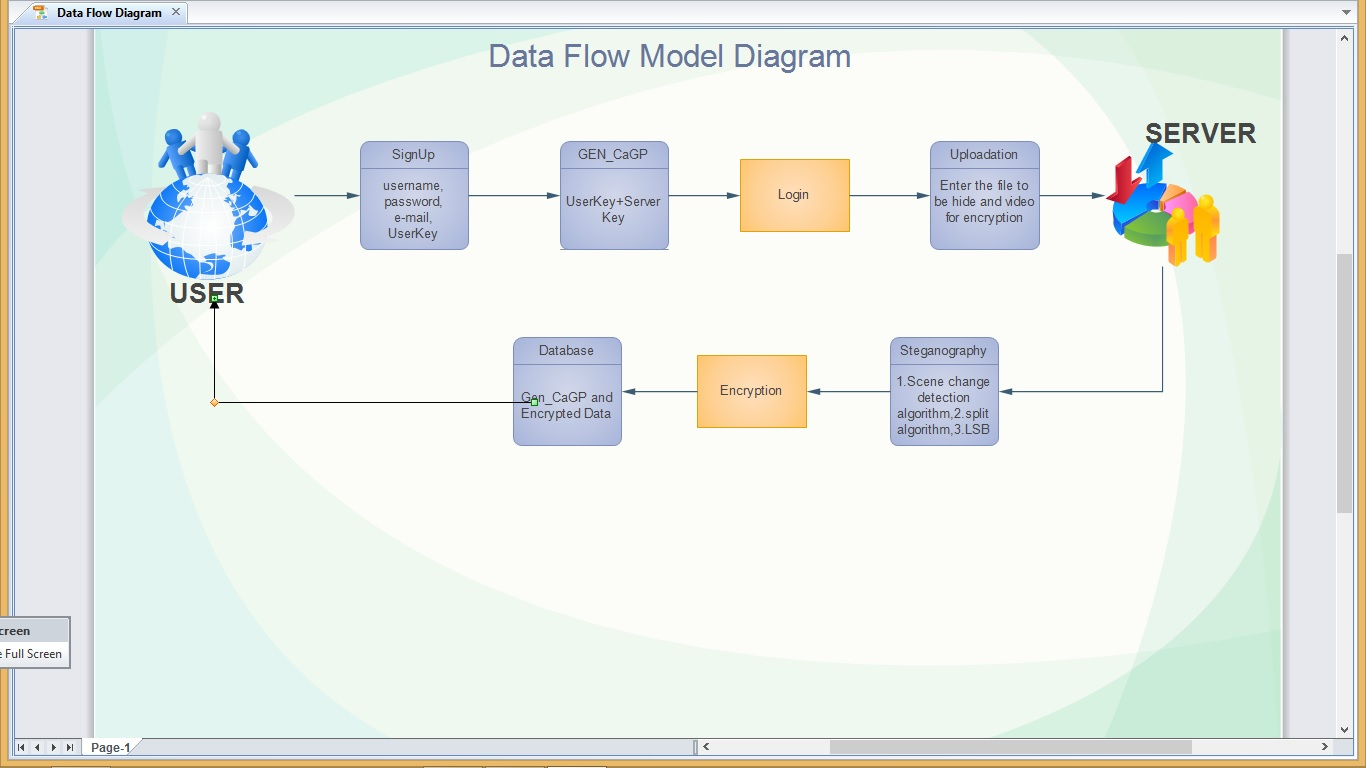
\includegraphics[scale=.45]{DFD.jpg}\\
  \caption{DFD Level}
  
\end{figure}

   %  \subsection{ENTITY RELATIONSHIP DIAGRAMS}
     \pagebreak
     \subsection{MATHEMATICAL MODEL}System Description:\newline
% Define block styles
\tikzstyle{decision} = [diamond, draw, fill=blue!20, 
    text width=4.5em, text badly centered, node distance=3cm, inner sep=0pt]
\tikzstyle{block} = [rectangle, draw, text width=5em, text centered, rounded corners, minimum height=4cm]
\tikzstyle{line} = [draw, -latex']
\tikzstyle{cloud} = [draw, circle, node distance=3cm,
    minimum height=2em]
    
    \textbf{Mathematical Model}\newline
    	       %\paragraph{}
    	       Let the M is the universal states which contains, \\
    \textbf{M = \{Q, S, F, Q0 , Qf \}} \newline
    where, \\
    		Q = No. of states \{Q0,Q1,Q2,Q3,Q4,Q5,Q6,Q7,Qf\}\\
    		Q0= Initial State.\\
    		Qf= Final State.\\
    		S= Success state.\\
    		F= Failure state.\\
    		\newline
		
    where,\\ 
    \newline
    Q0= Start.\\
     \newline
    Q1 = SignUp \\
    \newline
    Q2 = Generation of CaGP on Serverside\\
    \newline
    Q3 = Login\\
    \newline 
    Q4 = Verification of CaGP\\
    \newline
    Q5 = Select the data to be hidden\\
    \newline 
    Q6 = Select the file in which the data is to be hidden\\
    \newline
    Q7 = Steganography\\
    \newline 
    Qf = Encrypted data\\
    \newline 
    
    F = \{F,S\} \newline
    \newline Where ,
    \newline F  = Failure if the Username,Password or CaGp entered is incorrect\\
        \newline S = Successfully log in, Data is successfully Encrypted\\


    \section{Activity Diagram : }
\begin{tikzpicture}[node distance = 6cm, auto, line width=1pt,>=latex]
    % Place nodes
    \node [cloud] (Q0) {Q0};
    \node [cloud, right of=Q0] (Q3) {Q3};
    \node [cloud, below of=Q3] (Q1) {Q1};
    \node [cloud, right of=Q3] (Q4) {Q4};
    \node [cloud, below of=Q4] (Q2) {Q2};
    \node [cloud, right of=Q4] (Q5) {Q5};
    \node [cloud, right of=Q5] (Q6) {Q6};
    \node [cloud, below of=Q6] (Q7) {Q7};
    \node [cloud, below of=Q7] (Qf) {Qf};
    \node [cloud, below of=Q7] (Qf) {};
    
    % Draw edges
     \path [line] (Q0) -- (Q1);
    \path [line] (Q1) -- (Q2);
    \path [line] (Q2) -- (Q3);
    \path [line] (Q3) -- (Q4);
    \path [line] (Q4) -- (Q5);
    \path [line] (Q5) -- (Q6);
    \path [line] (Q6) -- (Q7);
    \path [line] (Q7) -- (Qf);
    \path [line] (Q0) -- (Q3);
    \end{tikzpicture} \\\\



  \newpage

\section{SYSTEM IMPLEMENTATION PLAN}

\begin{table}[ht]
\caption{System Implementation Plan Phase-I}
\begin{tabular}{ |M{2cm}|p{7cm}|M{2.5cm}|M{3.2cm}|  }
 \hline
 \textbf{SR. NO.} & \textbf{TASK NAME} & \textbf{DURATION} & \textbf{COMPLETION}\\
 \hline
 


  1. & Project Topic Selection &  15 days & $\checkmark$\\
  \hline
  2. & Literature Survey&  10 days& $\checkmark$\\
  \hline
  3. & Study Of Existing System  &  5 days & $\checkmark$\\
  \hline
  4. & Synopsis \& Abstract Submission  &  15 days & $\checkmark$\\
  \hline
   5. & SRS   &  15 days & $\checkmark$\\
   \hline
   6. & Design Of System Architecture &  5 days & $\checkmark$\\
  \hline
  7. & Design Of UML Diagrams  &  5 days & $\checkmark$\\
  \hline
    8. & Planning Of System Modules \& Interface &  8 days & $\checkmark$\\
  \hline
 
  
  
 
 \end{tabular}
 
\end{table}

\begin{table}[ht]
\caption{System Implementation Plan Phase-II}
\begin{tabular}{ |M{2cm}|p{7cm}|M{2.5cm}|M{3cm}|  }
 \hline
 \textbf{SR. NO.} & \textbf{TASK NAME} & \textbf{DURATION} & \textbf{COMPLETION}\\
 \hline
 
 9.& Implementation Of Login phase  &	10 Days	& \\
 \hline
 
10. &Implementation and generation CaGP &	10 Days	&\\
\hline

11. &Steganography 	& 10 Days& \\
\hline	
12.&scene change detection algorithm,split algorithm and LSB	&10 Days & \\
\hline
13. & Output Display &	8 Days	& \\
\hline
14. & Testing Of Above Modules After Completion of Each Module &	5 Days Per Module	& \\
\hline
15. & Project Review &	5 Days & \\
\hline



 
 \end{tabular}
 
\end{table}



%%%%%%%%%%%%%%%%%%%% CHAPTER 4 %%%%%%%%%%%%%%%%%%%%%

\chapter{SYSTEM DESIGN}

\section{SYSTEM ARCHITECTURE}
The overall system design consists of following modules:
\begin{enumerate}
\item SignUp phase
\item Login phase
\item Steganography
\end{enumerate}

\begin{figure}[H]


	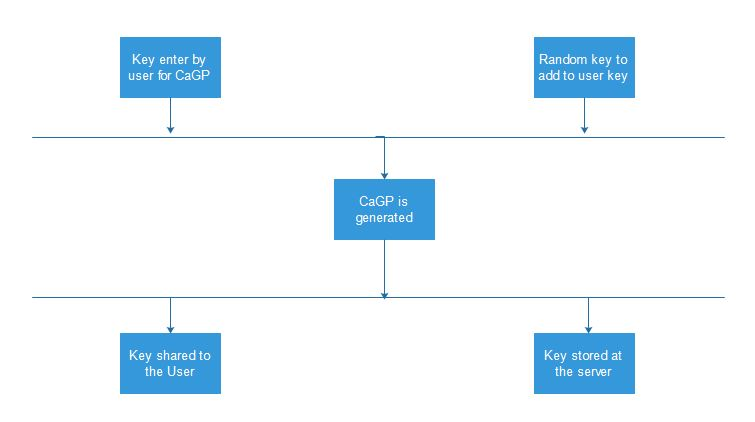
\includegraphics[scale=0.75]{1p.JPG}\\
	\caption{SignUp Phase}
	
	\end{figure}
	
	

\begin{figure}[H]


	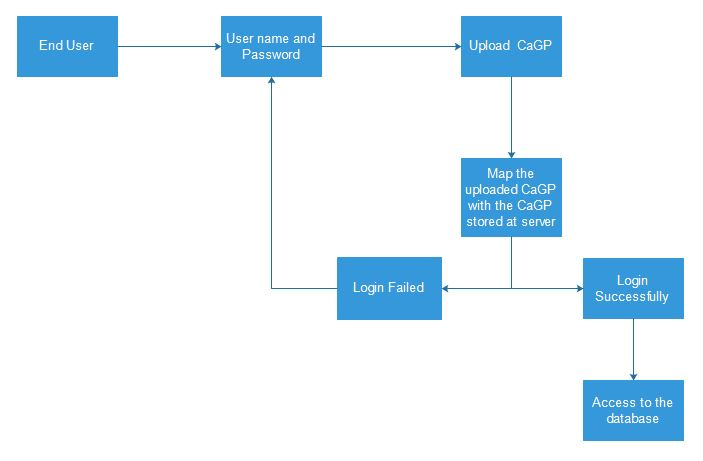
\includegraphics[scale=0.75]{2p.JPG}\\
	\caption{Login Phase}
	
	\end{figure}
	
	
	
\begin{figure}[H]


	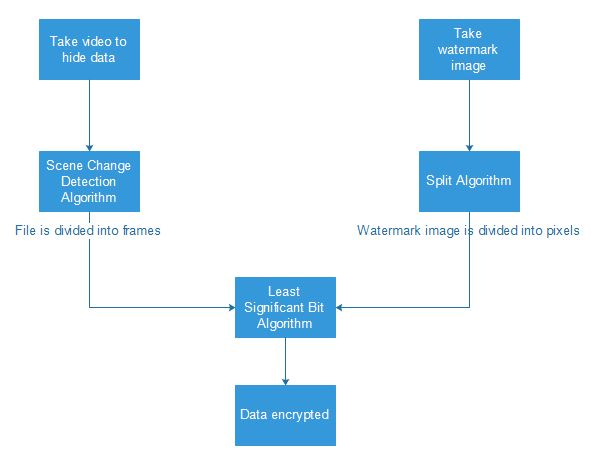
\includegraphics[scale=0.75]{3p.JPG}\\
	\caption{Steganography}
	
	\end{figure}


\hspace*{0.01em}
To work with this application first user needs to SignUp.In SignUp user needs to chose the Username and password along with this user need to enter email id and along with that tp generate the CaGP user need to enter a special key which contains the  string made of A-Z,a-z,0-9 combinations.At server side the key is generated by adding a random key which is made from combinations of A-Z,a-z,0-9 and then the key is generated in the form of CAPTCHA by using Visual cryptography.The generated CaGP is then mail to user for further process.Now for Login user need to its credentials along CaGP.
Now the entered CaGP is verified at server site,then user gets access to the application .
now user needs to upload the the data that he wants to hide,along with he needs to upload a file in which he wants to hide the data.
after uploading the data the actual process starts.Firstly the file in which the data is to be hide is broken into frames and a respective color histogram is form for each frame,its done by using SCENE CHANGE DETECTION ALGORITHM.
now the data which need to be hide is broken into the chunk by SPLIT ALGORITHM.After this the process of hiding the data starts with the leas significant bit




\section{UML DIAGRAMS}

\section*{\underline{Definition}}
\hspace*{5em}The Unified Modelling Language (UML) is a general purpose,developmental, modelling language in the field of software
engineering, that is intended to provide a standard way to visualize the design of a system. UML was originally motivated by the desire to standardize the disparate notational systems and approaches to software design.


\section*{\underline{Design}}
The Unified Modelling Language (UML) offers a way to visualize a system's architectural blueprints in a diagram  including elements such as:
\begin{itemize}


\item Any activities.
\item Individual components of the system:
And how they can interact with other software components.
\item How the system will run.
\item How entities interact with others (components and interfaces)
\item External user interface
\end{itemize}
\hspace*{5em}Although originally intended solely for object oriented design documentation, the Unified Modelling Language (UML) has been extended to cover a larger set of design documentation.


\section*{\underline{UML System Model}}
\begin{itemize}
\item \textbf{Static (or structural) view:}\\
Emphasizes the static structure of the system using objects, attributes,
operations and relationships. The structural view includes class diagrams and composite structure
diagrams.
\item \textbf{Dynamic (or behavioural) view:}\\
Emphasizes the dynamic behaviour of the system by showing collaborations among objects and changes to the internal states of objects. This view includes sequence diagrams, activity diagrams and state machine diagrams.
\end{itemize}

\section*{\underline{UML Models}}
\begin{enumerate}
\item \textbf{Use case diagram:}\\
To model a system the most important aspect is to capture the dynamic behaviour.
To clarify a bit in details, dynamic behaviour means the behaviour of the system when it is running /operating.
So only static behaviour is not sufficient to model a system rather dynamic
behaviour is more important than static behaviour.These internal and external agents are known as actors. So use case diagrams are consists of actors, use cases and their relationships. The diagram is used to model the system/subsystem of an application. A single use case diagram captures a particular functionality of a system.
So to model the entire system numbers of use case diagrams are used.
\item \textbf{Deployment Diagram:}\\
Deployment diagrams are used to visualize the topology of the physical
components of a system where the software components are deployed.
So deployment diagrams are used to describe the static deployment view of a system. Deployment diagrams consist of nodes and their relationships.
The name Deployment itself describes the purpose of the diagram. Deployment diagrams are used for describing the hardware components where software components are deployed. Component diagrams and deployment diagrams are closely related.
UML is mainly designed to focus on software artefacts of a system. But these two diagrams are special diagrams used to focus on software components and hardware components.So most of the UML diagrams are used to handle logical components but
deployment diagrams are made to focus on hardware topology of a system.
Deployment diagrams are used by the system engineers.
\item \textbf{Activity Diagram:}\\
Activity diagram is basically a flow chart to represent the flow form one activity toanother activity. The activity can be described as an operation of the system.So the control flow is drawn from one operation to another. This flow can be sequential, branched or concurrent. Activity diagrams deals with all type of flow control by using different elements like fork, join etc.
It captures the dynamic behaviour of the system. Other four diagrams are used to show the message flow from one object to another but activity diagram is used to show message flow from one activity to another.
It does not show any message flow from one activity to another. Activity diagram is some time considered as the flow chart. Although the diagrams looks like a flow chart but it is not. It shows different flow like parallel, branched, concurrent and single.

\noindent
\item \textbf{Sequence Diagram:}\\
A Sequence diagram is an interaction diagram that shows how processes operate with
one another and in what order. It is a construct of a Message Sequence Chart. A sequence
diagram shows object interactions arranged in time sequence. It depicts the objects
and classes involved in the scenario and the sequence of messages exchanged between
the objects needed to carry out the functionality of the scenario. Sequence diagrams
are typically associated with use case realizations in the
Logical View of the system under development. Sequence diagrams are sometimes called
event diagrams or event scenarios.
A sequence diagram shows, as parallel vertical lines (lifelines), different processes
or objects that live simultaneously, and, as horizontal arrows, the messages exchanged between them, in the order in which they occur. This allows the specification of simple runtime scenarios in a graphical manner.

\item \textbf{State Chart Diagram:}\\
The name of the diagram itself clarifies the purpose of the diagram and other details. It describes different states of a component in a system. The states are specific to a component/object of a system. A State chart diagram describes a state machine. Now to clarify it state machine can be defined as a machine which defines different states of an object and these states are controlled by external or internal events. Activity diagram explained in next chapter, is a special kind of a State chart diagram. As State chart diagram defines states it is used to model lifetime of an object. State chart diagram is one of the five UML diagrams used to model dynamic nature of a system. They define different states of an object during its lifetime. And these states are changed by events. So State chart diagrams are useful to model reactive systems. Reactive systems can be defined as a system that responds to external or internal events. State chart diagram describes the flow of control from one state to another state. States are defined as a condition in which an object exists and it changes when some event is triggered.

\newpage
\item \textbf{Class Diagram:}\\
In software engineering, a class diagram in the Unified Modelling Language (UML) is a type of
static structure diagram that describes the structure of a system by showing the system's classes, their attributes, operations (or
methods), and the relationships among objects.The class diagram is the main building block of object oriented modelling. It is used both for general
conceptual modelling of the systematics of the application, and for detailed modelling translating the models into programming code. Class diagrams can also be used for data modelling.In the diagram, classes are represented with boxes which contain
three parts as follows the top part contains the name of the class, the middle part contains the attributes of the class and the bottom part contains the methods the class can execute.\\

\end{enumerate}

\pagebreak
    \subsection{USE CASE DIAGRAM}
    \begin{figure}[H]
    \centering
  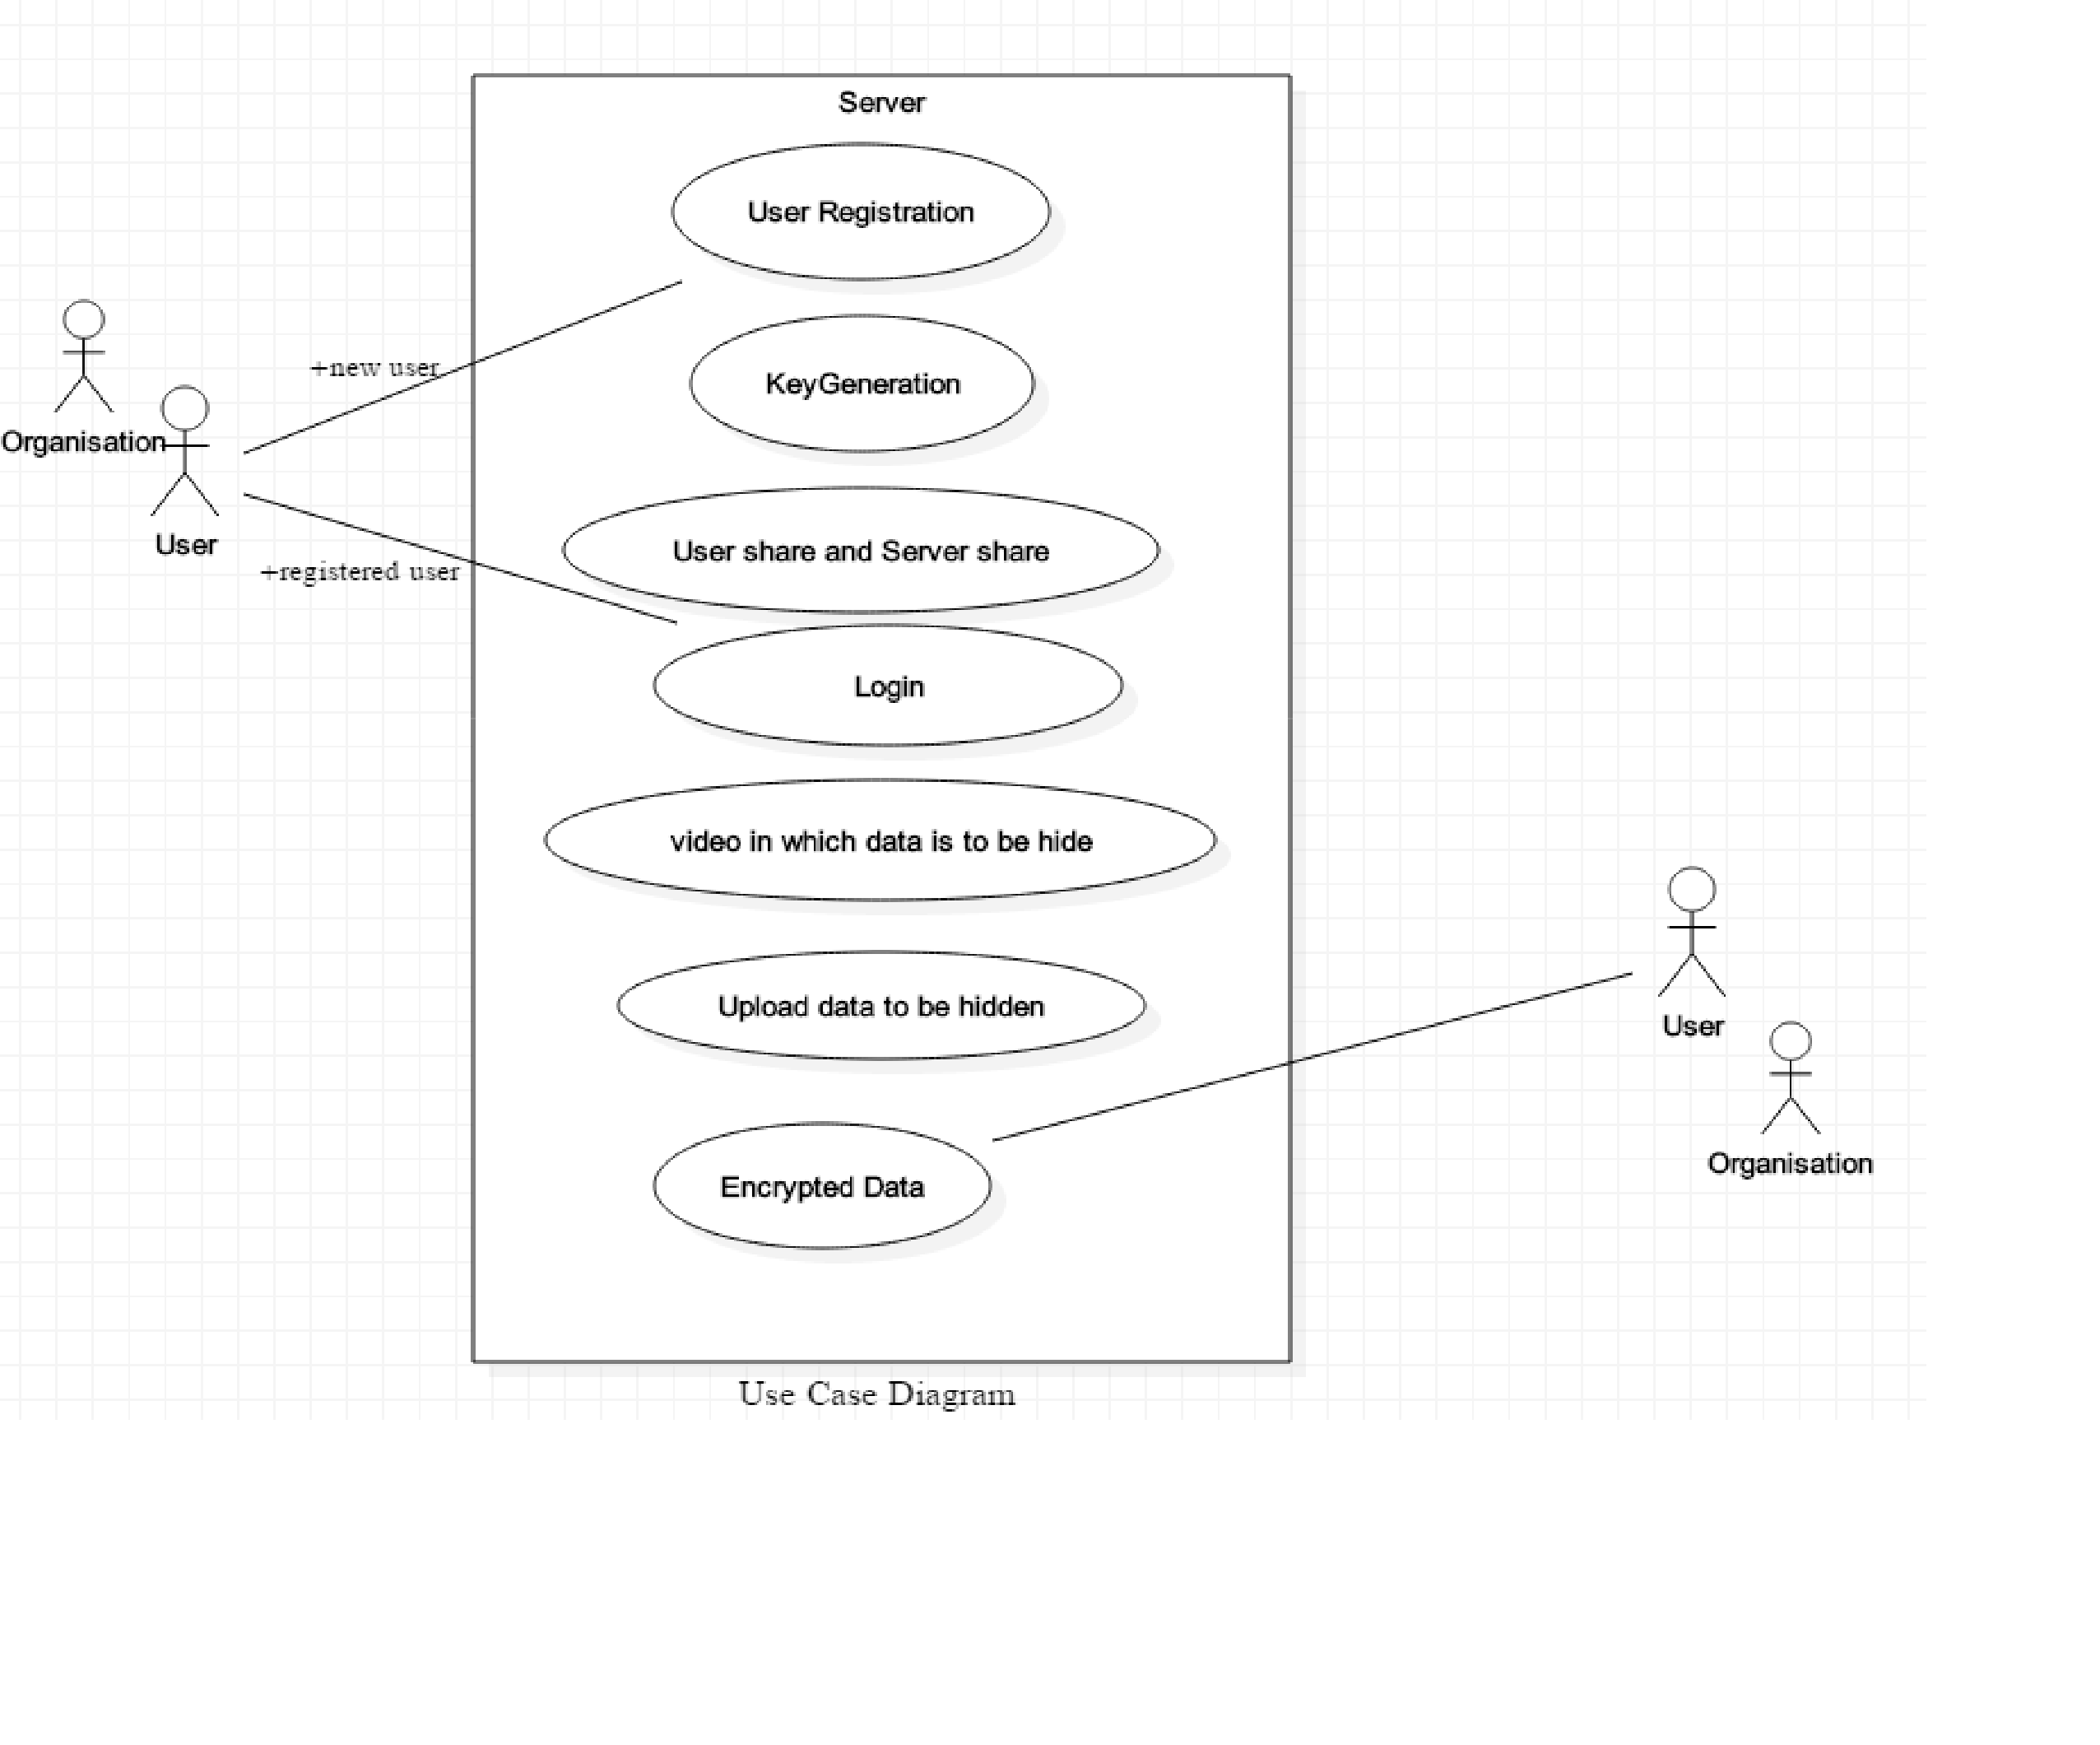
\includegraphics[scale=0.2]{usecase.png}
  \caption{Use Case Diagram}
  
\end{figure}
    \pagebreak
    \subsection{DEPLOYMENT DIAGRAM}
     \begin{figure}[H]
  \centering
  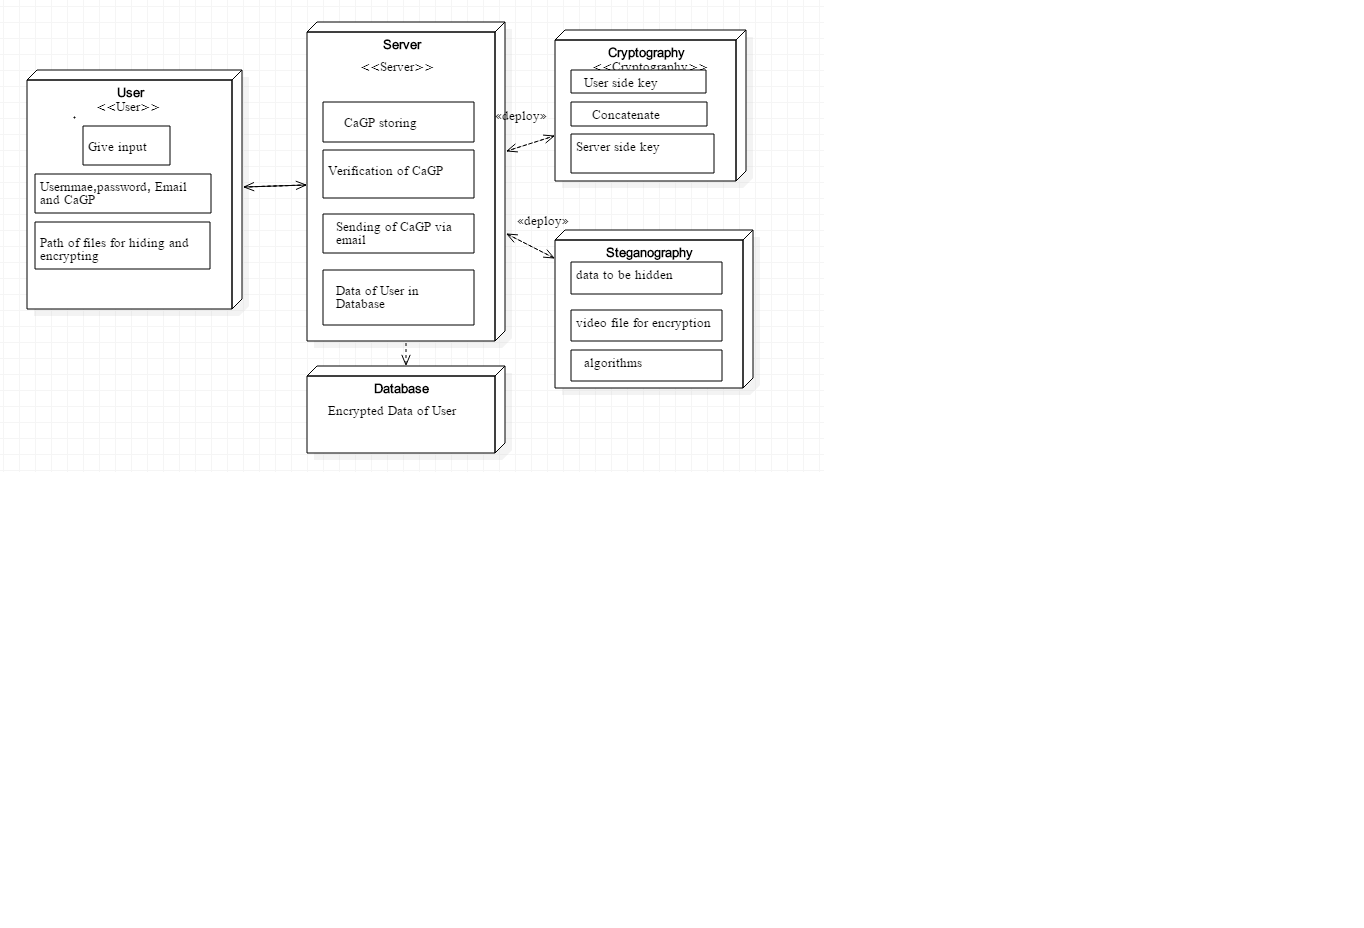
\includegraphics[scale=0.5]{deployment.png}\\
  \caption{Deployment Diagram}
  \end{figure}
  \pagebreak  
    \subsection{ACTIVITY DIAGRAM}
    \begin{figure}[H]
  %\centering
  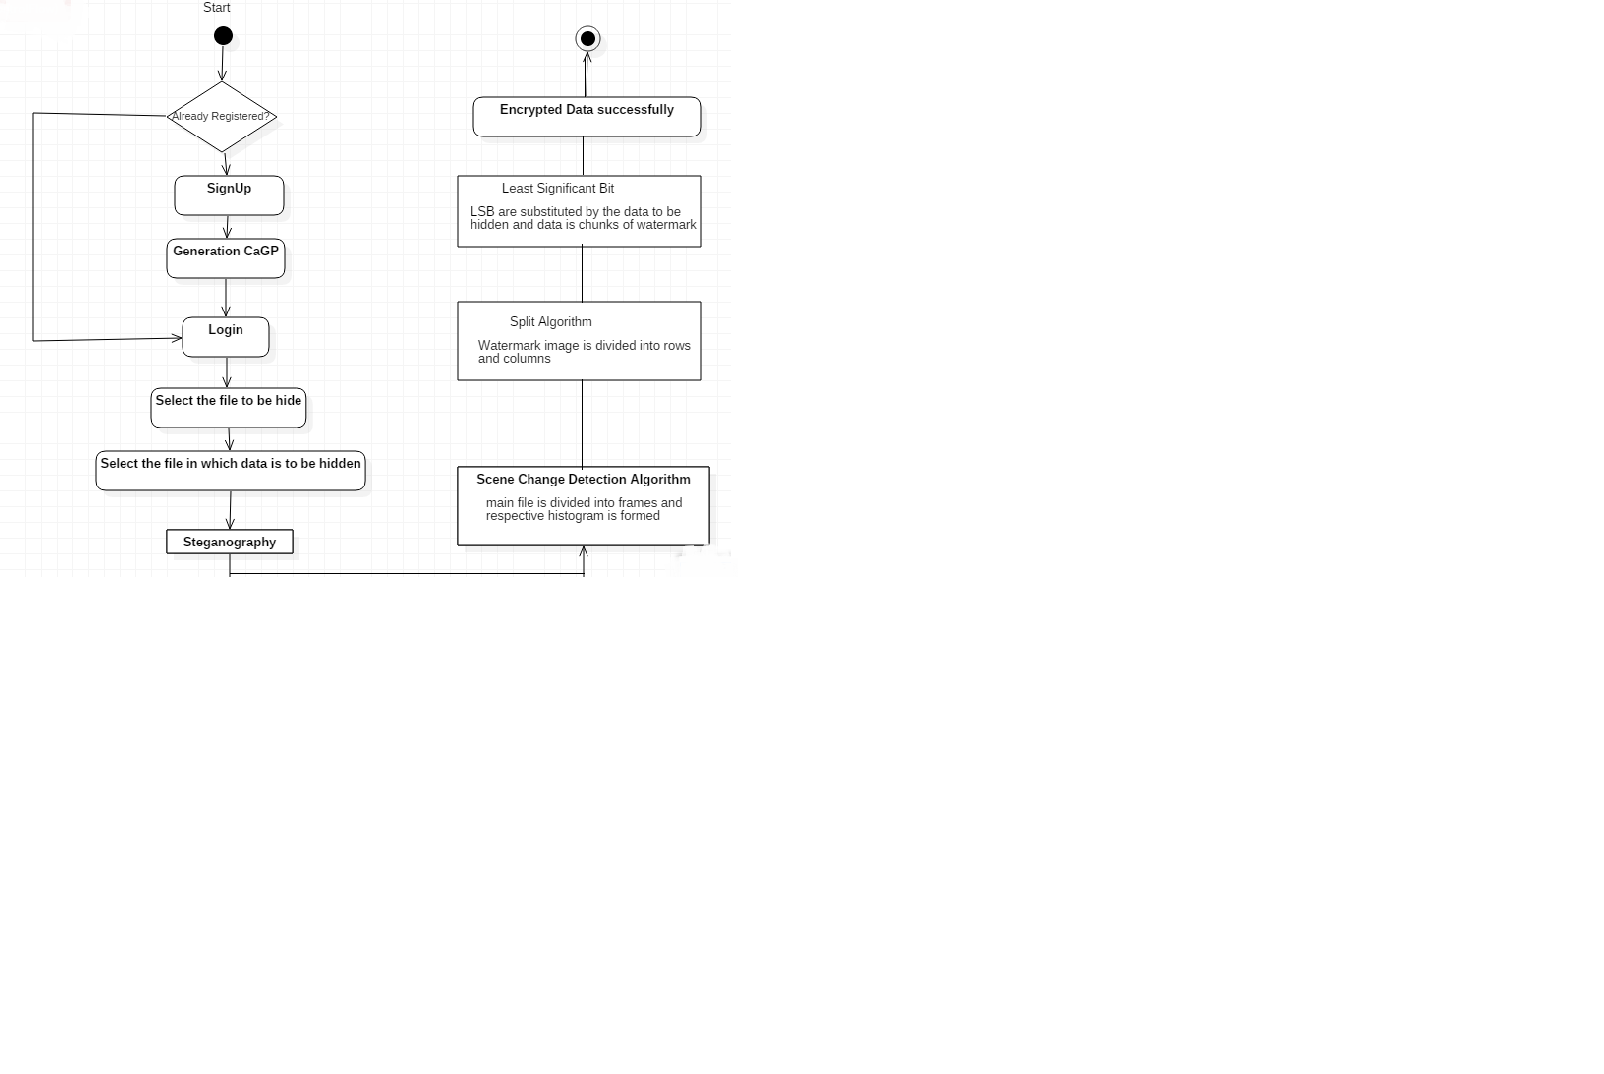
\includegraphics[scale=0.7]{activ.png}\\
  \caption{Activity Diagram}
  
\end{figure}
    
   \pagebreak 
    \subsection{SEQUENCE DIAGRAM}
    \begin{figure}[H]
  \centering
  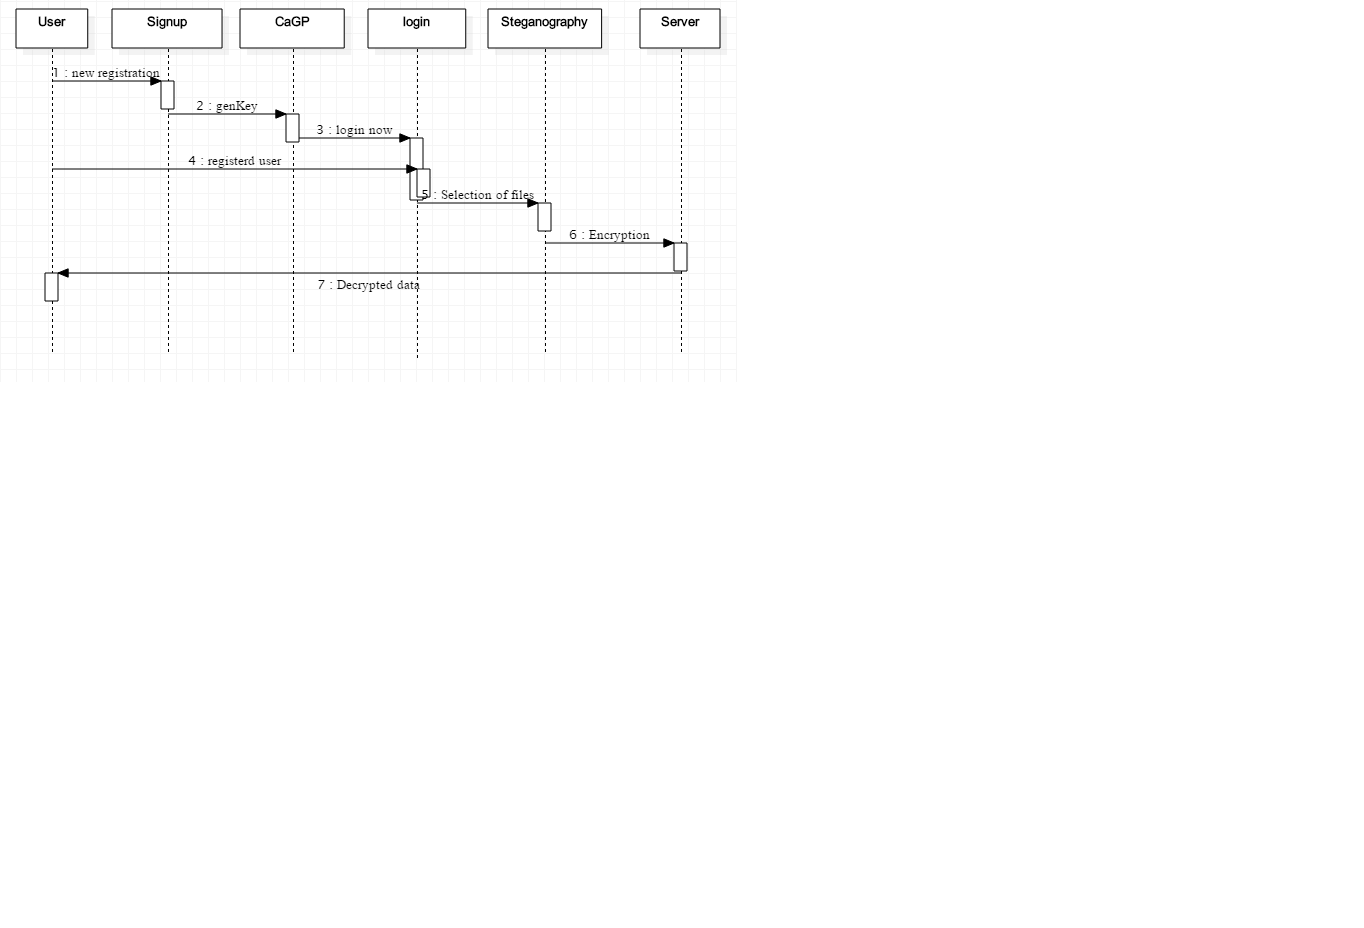
\includegraphics[scale=0.75]{sequence.png}\\
  \caption{Sequence Diagram}
  
\end{figure}
 \pagebreak   
    \subsection{STATE CHART DIAGRAM}
    
    \begin{figure}[H]
  \centering
  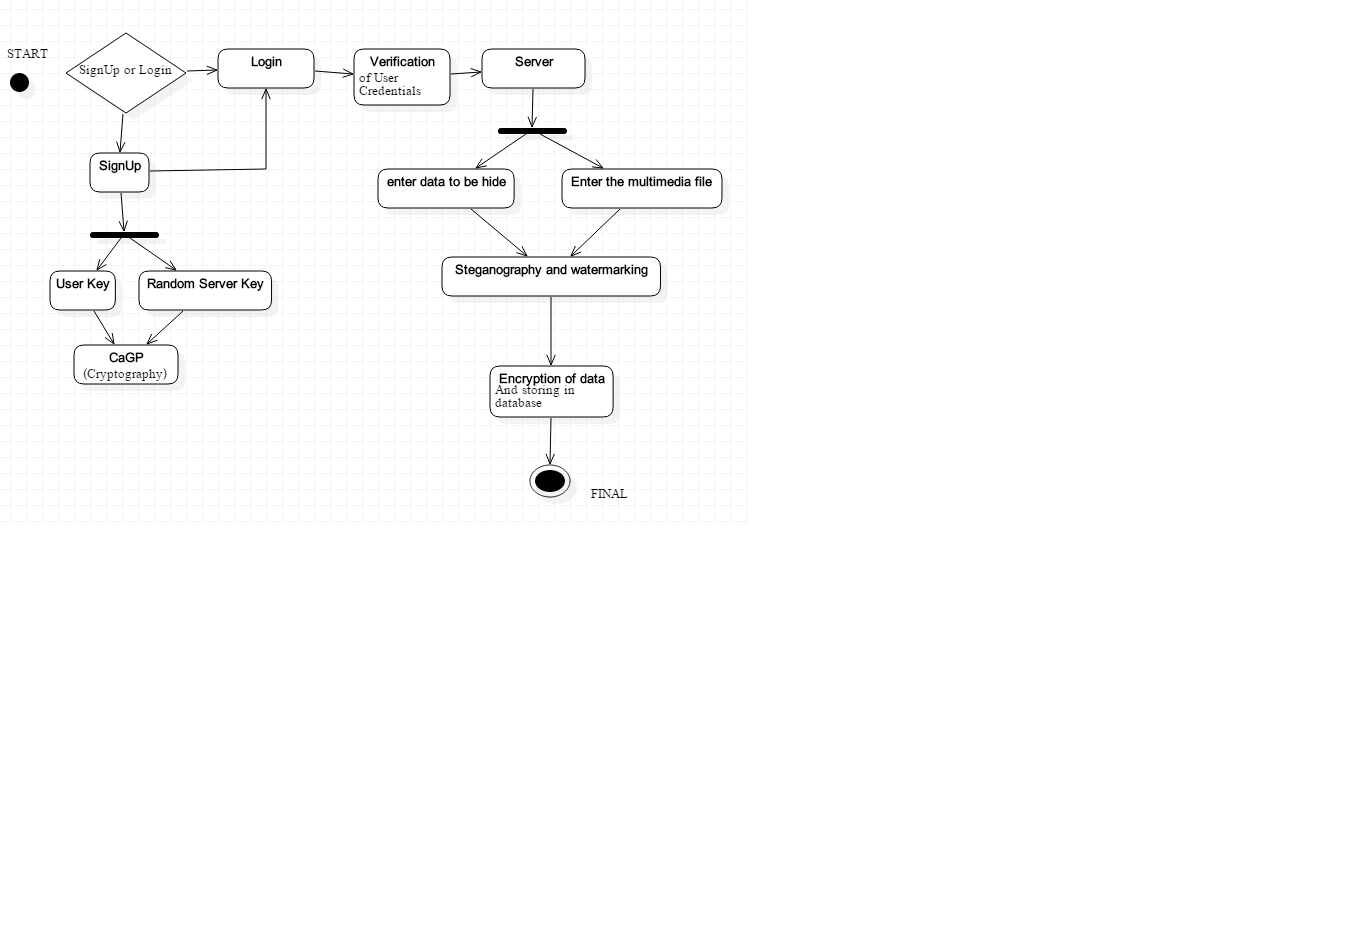
\includegraphics[scale=0.7]{State.png}\\
  \caption{State Chart Diagram}
  
\end{figure}
\pagebreak
    \subsection{CLASS DIAGRAM}
    \begin{figure}[H]
    \centering
  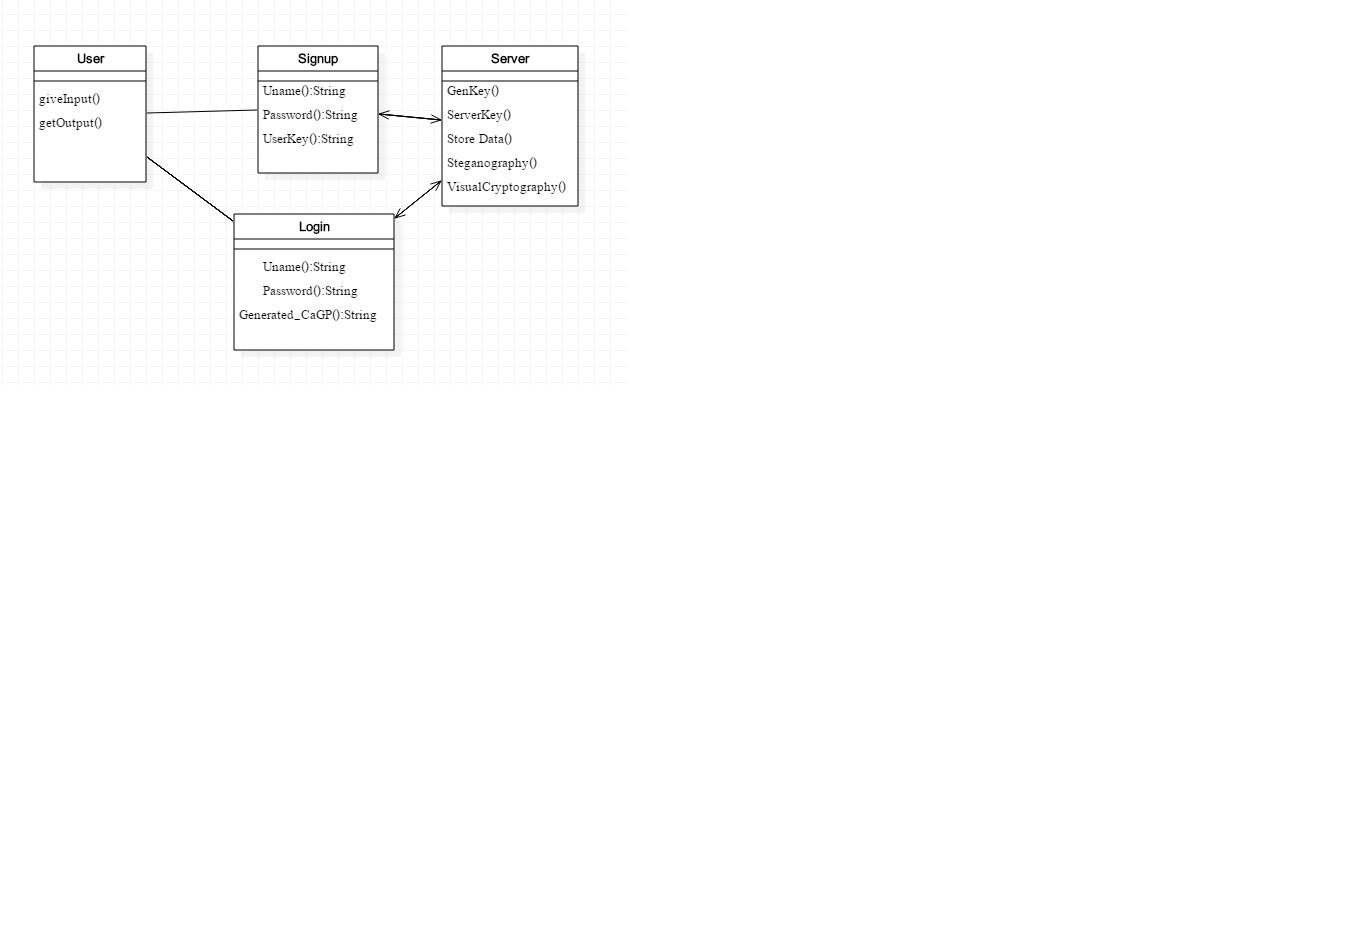
\includegraphics[scale=0.75]{Class.png}\\
  \caption{Class Diagram}
  
\end{figure}
%%%%%%%%%%%%%%%%%% CHAPTER 5 %%%%%%%%%%%%%%%%%%%%%%
\chapter{TECHNICAL SPECIFICATION}

\section{ADVANTAGES}
\begin{itemize}

\item User Friendly.
\item Secure Login to Database.
\item Huge size of data can be uploaded.
\item Secrecy in terms of hiding files.
\item Accurate Extraction.
\item Resistance from External Attacks.
\item Internet Rectified System.
\end{itemize}
\section{DISADVANTAGES}
\begin{itemize}


 \item 	Small alteration in files.
 \item Complication for Recovery of files.
 \item Time Consuming to decipher.
 \item Technical Difficulties 
\end{itemize} 
\newpage
 \section{APPLICATIONS}
\begin{itemize}

\item Alleged use in intelligence services
\item Confidential communicaions and secret data storing.
\item Media database system
\item Printer Steganography
\item Huge scope in military applications
\end{itemize}
%%%%%%%%%%%%%%%%%% CHAPTER 6 %%%%%%%%%%%%%%%%%%%%%%%
\chapter{RESULTS}
\section{EXPECTED RESULTS}
\hspace*{5em}Application will be able to successfully the encrypt the data into the file with the help of data provided by user.the data generated is not easy to detect normal humans eyes and it provide security from intruders and hackers.Because of the modified Login system, the system will be more secure than previous one and the valuable data of user will not be compromised.

\chapter{CONCLUSION}
\hspace*{5em}\\The application that we have build has a more secure Login system and data is protected from intruders and hackers.The data that user want to keep safe,secure and preserve is done by hiding it in in another file without destroying the file used to hide.The safety measures ,legals are all maintain without exploiting the rules.

Thus, on the basis of literature survey and by analysing the existing system, we have came to a conclusion that the proposed system will not only provide the secured Login to system but also it will help to keeps its data safe.


\renewcommand{\bibname}{REFERENCES}
\begin{thebibliography}{11}
\bibitem{DE} Shiju Sathyadevan, Devan M.S and Surya Gangadharan. S., \lq\lq Crime Analysis and Prediction Using Data Mining", Published in 2014 First International Conference on Networks \& Soft Computing, ISBN - 978-1-4799-3486-7 114-2014 IEEE 
\bibitem {} Isuru Jayaweera, Chamath Sajeewa, Sampath Liyanage, Tharindu Wijewardane, Indika Perera and Adeesha Wijayasiri, \lq\lq Crime Analytics: Analysis of Crimes Through Newspaper Articles", ISBN - 978-1-4799-1740-2/15 2015 IEEE

\bibitem {} Hsinchun Chen Wingyan Chung Jennifer Jie Xu Gang Wang Yi Qin and Michael Chau,\lq\lq Crime Data Mining: A General Framework and Some Examples", Published by the IEEE Computer Society ,ISBN - 0018-9162/04/2004 IEEE
\bibitem{} GU Yunhua, SHEN Shu, ZHENG Guansheng,\lq\lq Application of NoSQL Database in Web Crawling", International Journal of Digital Content Technology and its Applications. Volume 5, Number 6, June 2011.
\bibitem {} S.L. Ting, W.H. Ip, Albert H.C. Tsang, \lq\lq Is Naive Bayes a Good Classifier for Document Classification?", International Journal of Software Engineering and Its Applications Vol. 5, No. 3, July, 2013.
\bibitem {} Anagha R Kulkarni, Vrinda Tokekar, Parag Kulkarni,\lq\lq Identifying Context of Text Documents using Naive Bayes Classification and Apriori Association Rule Mining",IET, Devi Ahilya University, Khandawa Road, Indore 452017, India cEKlat Research, Pune, India.
\bibitem{} Mohammed Al-Maolegi1, Bassam Arkok, \lq\lq AN IMPROVED APRIORI ALGORITHM FOR ASSOCIATION RULES",Published in International Journal on Natural Language Computing (IJNLC) Vol. 3, No.1, February 2014.
\bibitem{} Wei Peng, Juhua Chen and Haiping Zhou,\lq\lq An Implementation of ID3 - Decision Tree Learning Algorithm" Project of Comp 9417: Machine Learning University of New South Wales, School of Computer Science\& Engineering, Sydney, NSW 2032, Australia.
\end{thebibliography}

\newpage
\appendix
\chapter{GLOSSARY}
\begin{table}[ht]
\centering
\begin{tabular}{ |M{3cm}|p{8cm}|  }
 \hline
\textbf{CAPTCHA}& Completely Automated Public Turing Test To Tell Computers And  Humans Apart\\
\hline
\textbf{CaGP} &CAPTCHA As Graphical Password\\
\hline
\textbf{JDK} & Java Development Kit\\
\hline
\textbf{GUI} & Graphical User Interface\\
\hline
\textbf{IDE} & Integrated Development Environment \\
\hline
\textbf{UML} & Unified Modelling Language\\
\hline
\textbf{DB}&  DataBase\\
\hline


\end{tabular}

\end{table}


\chapter{ASSIGNMENTS}
\vspace{0.5}
\section*{\centering\LARGE{Lab Assignment 01}}

\subsection*{\underline{Aim}}
Refer Chapter 7 of first reference to develop the problem under consideration and justify feasibility using concepts of knowledge canvas and IDEA Matrix. 
\subsection*{\underline{Project}}
Database security using Image Captcha as Graphical Password(CaGP) and Steganography.\\
\begin{table}[ht]
\caption{Project Canvas}
\begin{tabular}{ |p{5cm}|p{5cm}|p{5cm}|  }
 \hline
 \textbf{Purpose} & \textbf{Goals} & \textbf{Users}\\
 \hline
To increase safety and security & Increase the security for (captcha) Verification & Banking Sector\\

To hide data securely in video format & Store data  in video format & Verification Analysts\\
 \hline
 \end{tabular}
 \vspace{0.5cm} 
 
\begin{tabular}{ |p{5cm}|p{5cm}|p{5cm}|  }
 \hline
 \textbf{Actions} & \textbf{Deliverables} & \textbf{Risks} \\
 \hline
 Verification Login  & SRS  \& Project Design & DB may get compromised\\


  Analyze input data & Project Report \& Project & DB may leads to system error\\
   \hline
 
 \end{tabular}
 
\vspace{0.5cm} 

 \begin{tabular}{ |p{5cm}|p{5cm}|p{5cm}|  }
 \hline
 \textbf{Milestones} & \textbf{Constraints} & \textbf{Scope} \\
 \hline
 Synopsis, Abstract, Report & Input to be stored in DB & Concurrent Processing\\

  Coding and Final Software & Software must meet minimum system requirement & Password Protection \\ 
   \hline
 
 \end{tabular}

\end{table} \\\\
\pagebreak
\newpage
\noindent\\\\
\\\\
\\\\
\\\\
\\\\
\\\\
\\\\
\\\\
\\\\
\\\\
\\\\
 \newpage
\section*{\centering\LARGE{Lab Assignment 02}}
\subsection*{\underline{Aim}}
Project problem statement feasibility assessment using NP-Hard, NP-Complete or satisfy ability issues using modern algebra and/or relevant mathematical models.

\subsection*{\underline{Feasibility Theory}}
The feasibility of the project can be defined as the measure of our project whether it is viable or not.It includes various different types of feasibility as follows:
\begin{itemize}
\item \textbf{Performance:}\\
In this we check whether the proposed system is capable of performing all the functional requirements as mentioned in system features in SRS.If our system is displaying the functional requirements appropriately then it's performance is feasible.Here we also check the accuracy and efficiency of the system based on their algorithms.
\item \textbf{Technical:}\\
In this we check whether the technical specification provided that is hardware and software requirements are minimum requirements for our application software to run successfully without any error regarding the system configuration.Also the  storage requirements is quite enough and concurrency takes place effectively.
\item \textbf{Economical:}\\
In this we check the cost per line of code also the cost for storage of data and cost related to the run time of the system.Apart from this since no extra hardware is needed apart from minimum system configuration for the computers on network.


\end{itemize}
\noindent
\subsection*{\underline{Feasibility on basis of Class of Problem}}
\hspace{5em}Complexity classes are one way to talk about how difficult or easy a problem is.
Complexity theory gets very technical but the basics are actually extraordinarily
intuitive, and it's possible to understand the P versus NP issue with very little
math background.\\

\hspace{1em}If there is a fast solution to the search version of a problem then the problem is
said to be Polynomial time,
or P for short. If there is a fast solution to the verification version of a problem then the problem is said to be
Non deterministic Polynomial time,
or NP for short. The question of
"P=NP" is then the question of whether these sets are identical.\\

\hspace{1em}Some problems can be translated into one another in such a way that a fast
solution to one problem would automatically give us a fast solution to the
other. There are some problems that every single problem in NP can be
translated into, and a fast solution to such a problem would automatically give
us a fast solution to every problem in NP. This group of problems are known as
NP Hard.Some problems in NP Hard
are actually not themselves in NP,the
group of problems that are in both NP and NP Hard
is called NP Complete

\subsection*{\underline{Classes of problems}}
\begin{itemize}
\item \textbf{NP}\\
A lot of programs that don't (necessarily) run in polynomial time
on a regular computer, but do run in polynomial time on a non deterministic
Turing machine. These programs solve problems in NP, which stands for
non deterministic polynomial time.An equivalent way to define NP is by pointing to the problems that can be
verified in polynomial time.

\item \textbf{NP Hard}\\
If a problem is NP hard,
this means I can reduce any problem in NP to that problem. This means if I can solve that problem, I can easily solve any problem in NP. If we could solve an NP hard
problem in polynomial time, this would
prove P = NP.

\item \textbf{NP Complete}\\
A problem is NP complete
if the problem is both
NP hard, and in NP
\end{itemize}
\noindent
\hspace{5em}Our project  is  divided  into  two  parts.   First  part  is  login  phase  using  vi- sual cryptography scheme and second part is watermarking for upload and download data with video watermark.  As we are providing security to both login phase and data, it should not be in NP hard or np.  Our vcs algorithm will not go in infinite loop or it will not cause system to get stand by.
Same thing will happen for watermarking algorithms also.  Output of this
system will definitely come but time will not same for each output hence it is in np complete.

\subsection*{\underline{Relation Between Classes of Problems}}
 \begin{figure}[H]
    \centering
  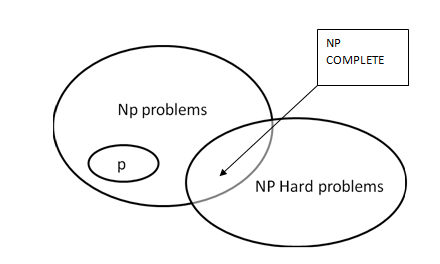
\includegraphics[scale=0.9]{np.PNG}\\
 \caption{Relation between Classes of Problems}
  
\end{figure}

\subsection*{\underline{Mathematical Model}}
 Let the M is the universal states which contains, \\
    \textbf{M = \{Q, S, F, Q0 , Qf \}} \newline
    where, \\
    		Q = No. of states \{Q0,Q1,Q2,Q3,Q4,Q5,Q6,Q7,Qf\}\\
    		Q0= Initial State.\\
    		Qf= Final State.\\
    		S= Success state.\\
    		F= Failure state.\\
    		\newline
		
    where,\\ 
    \newline
    Q0= Start.\\
     \newline
    Q1 = SignUp \\
    \newline
    Q2 = Generation of CaGP on Serverside\\
    \newline
    Q3 = Login\\
    \newline 
    Q4 = Verification of CaGP\\
    \newline
    Q5 = Select the data to be hidden\\
    \newline 
    Q6 = Select the file in which the data is to be hidden\\
    \newline
    Q7 = Steganography\\
    \newline 
    Qf = Encrypted data\\
    \newline 
    
    F = \{F,S\} \newline
    \newline Where ,
    \newline F  = Failure if the Username,Password or CaGP entered is incorrect\\
        \newline S = Successfully log in, Data is successfully Encrypted\\






\newpage
\section*{\centering\LARGE{Lab Assignment 03}}
\subsection*{\underline{Aim}}
Use of divide and conquer strategies to exploit distributed/parallel/concurrent processing of the above to identify objects, morphisms, overloading in functions (if any), and functional relations and any other dependencies (as per requirements).
\subsection*{\underline{Concept}}
A divide and conquer algorithm works by recursively breaking down a problem into two or more sub-problems of the same (or related) type (divide), until these become simple enough to be solved directly (conquer). So have divided our problem based on algorithm used and those are:
\begin{itemize}
\item Getting data from user.
\item Scene Change Detection(Compare 2 frames based on their color histogram)
\item Split Algorithm(Decide number of rows and columns to split the watermark image)
\item Least Significant Bit Algorithm(few least significant bits are substituted within data to be hidden)
\end{itemize}

\vspace*{0.4cm}
\noindent
\hspace{5em}Divide and conquer (D\&C) is an algorithm design paradigm based on multi-branched recursion. So we have to recursively divide our problem into  sub-problems  of the same (or related) type (divide), until these sub-problem become simple enough to be solved directly (conquer). The solutions to the sub-problems are then combined to give a solution to the original problem.\\

%\vspace*{0.4cm}
\noindent
\hspace{5em}In our project we are using a similar but with a slight difference in Divide and Conquer strategies in Scene change detection algo and split algo.In scene change algo we are the dividing the the file e.g video into frames and making the histograms of each frame.If the change in actual frame and the frame of the encrypted file is above the threshold then the scene is vchanged and the file is again processed until it match threshold level.
        same in case of split algo the data or the watermarke image to be hidden is divided into chunks.Number of rows and columns are decided to slit the watermark.
\newpage
\noindent
\textbf{System Specifications and Dependencies}\\
The system comprises of following major components : 
\begin{itemize}


\item SignUp/Register and Login :- take input from files.
\item Compare 2 frames based on their color histogram
\item Decide number of rows and columns to split the watermark image
\item few least significant bits are substituted within data to be hidden.
\end{itemize}

 

\newpage
\section*{\centering\LARGE{Lab Assignment 04}}
\subsection*{\underline{Aim}}
Use of above to draw functional dependency graphs and relevant Software modelling methods, techniques including UML diagrams or other necessities using appropriate tools.
    \subsection*{USE CASE DIAGRAM}
    \begin{figure}[H]
    \centering
  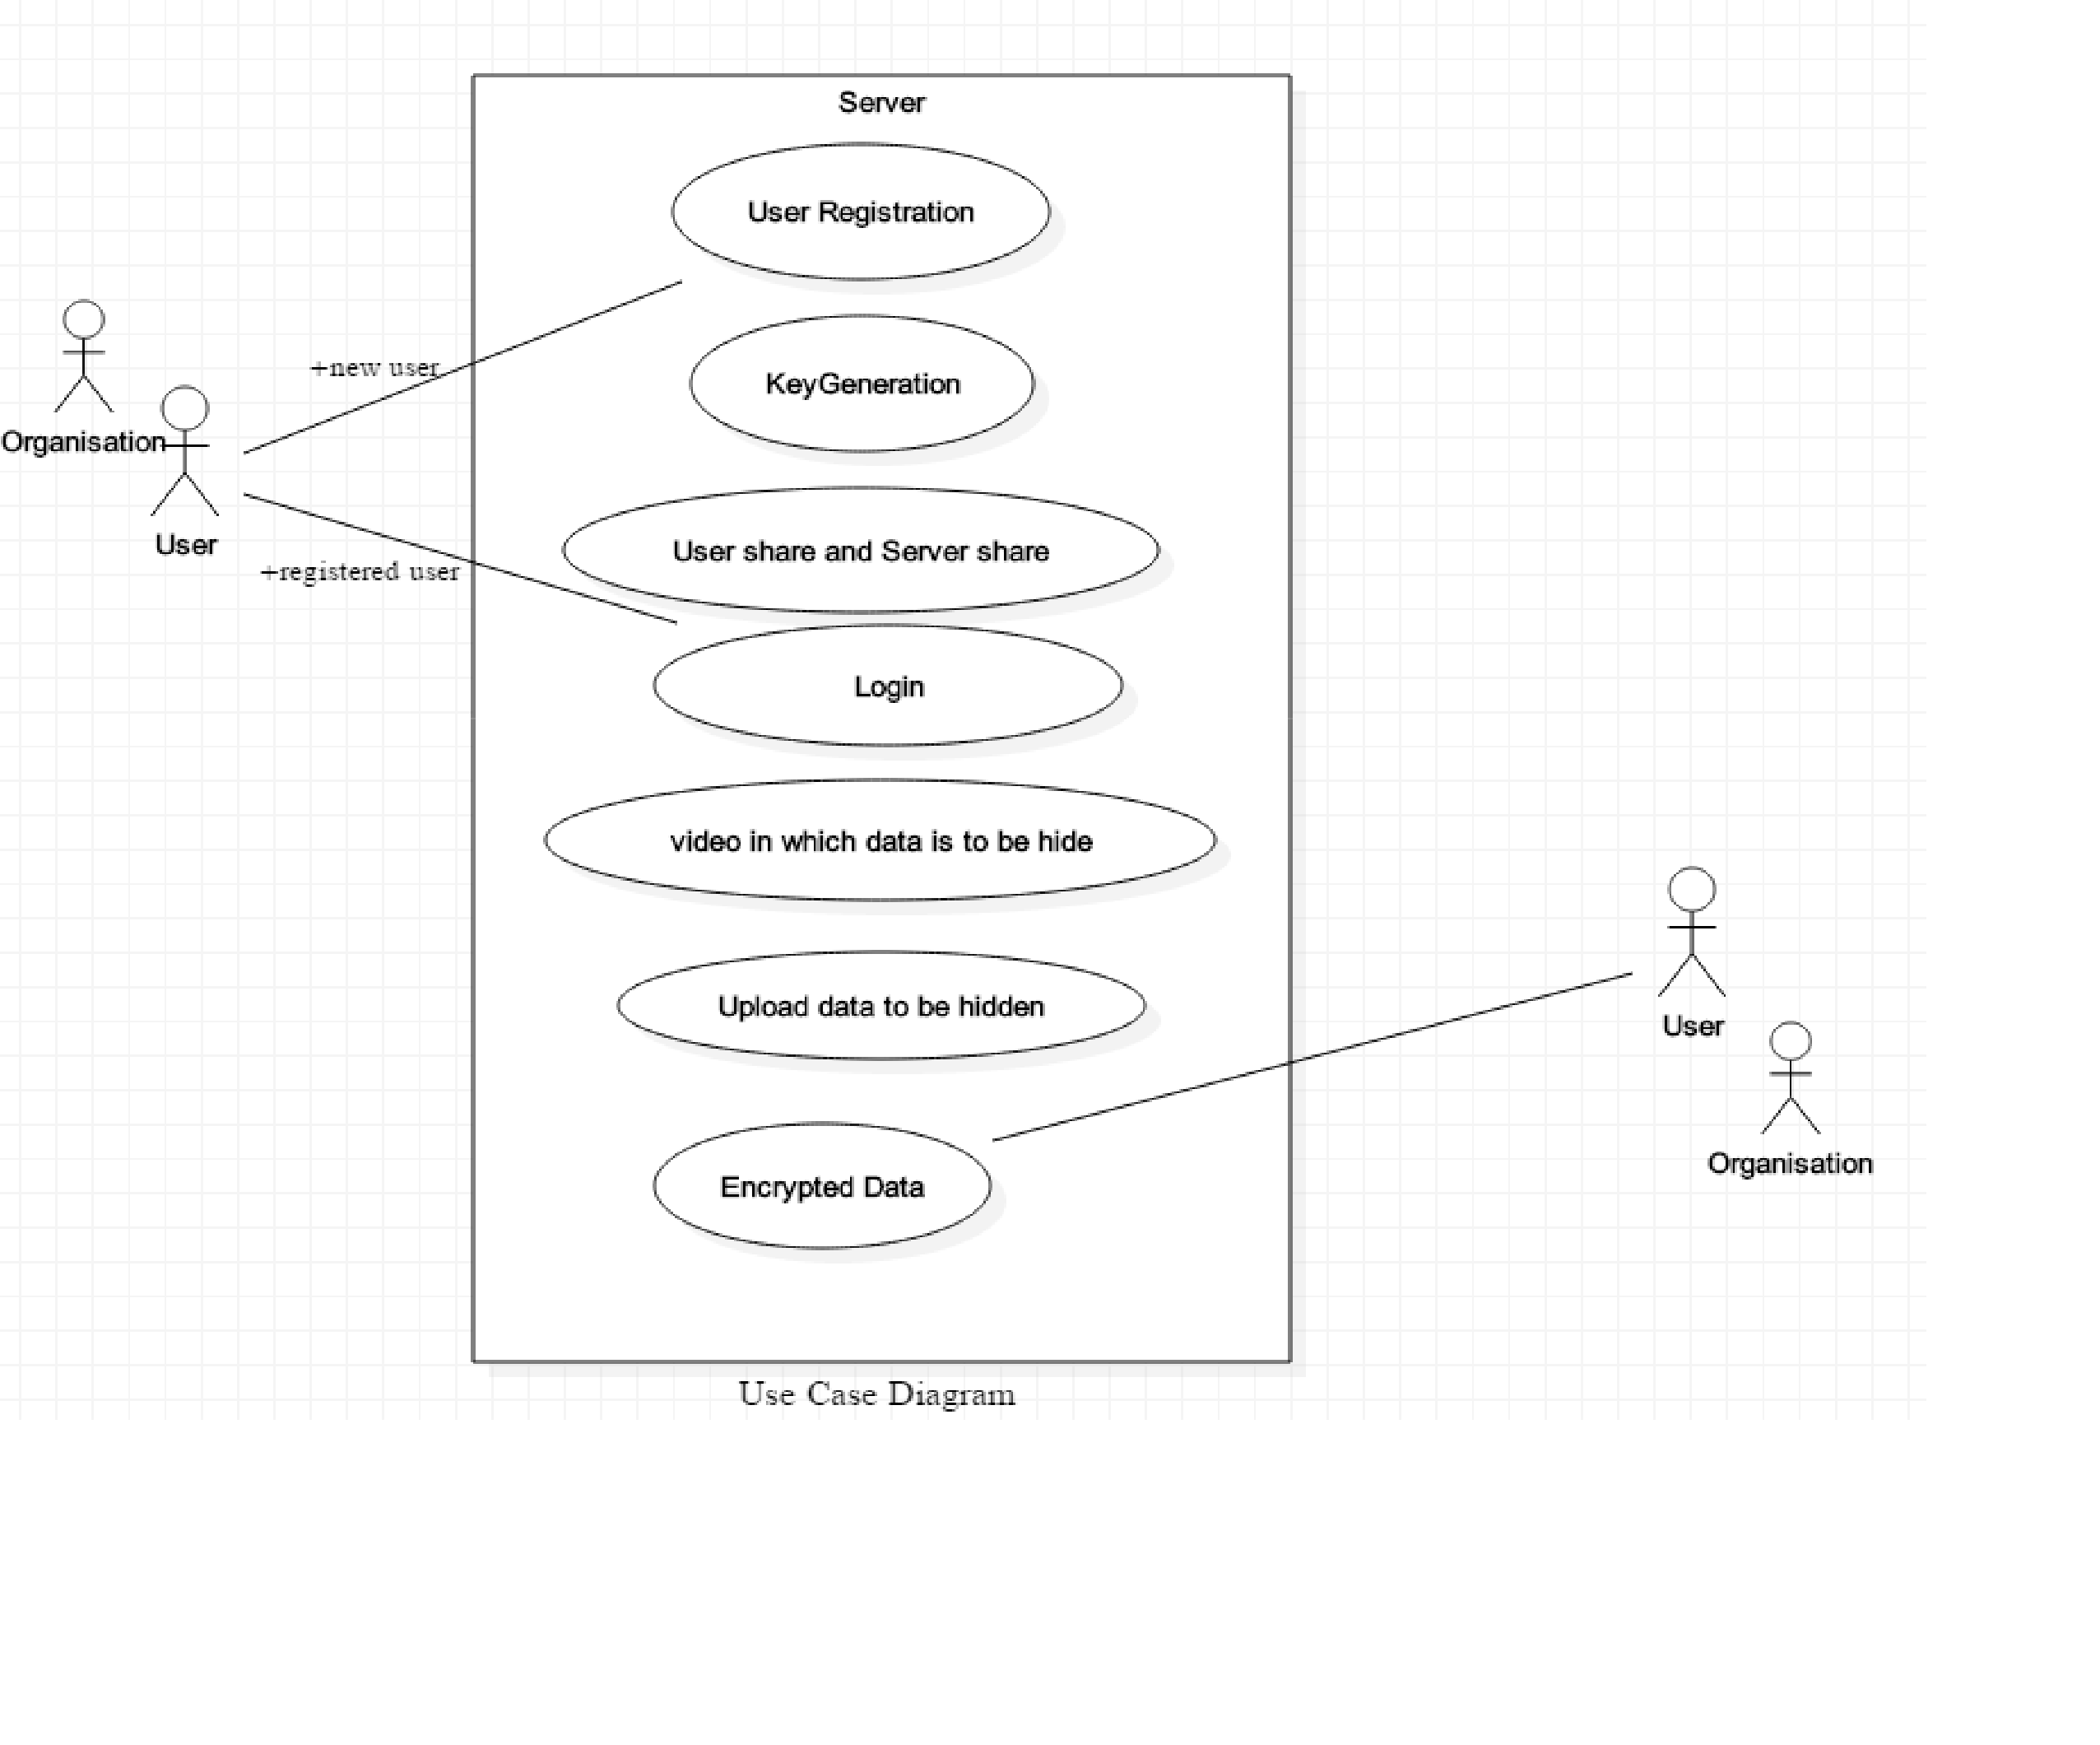
\includegraphics[scale=0.25]{usecase.png}\\
  \caption{Use Case Diagram}
  
\end{figure}
    \pagebreak
    \subsection*{DEPLOYMENT DIAGRAM}
     \begin{figure}[H]
  \centering
  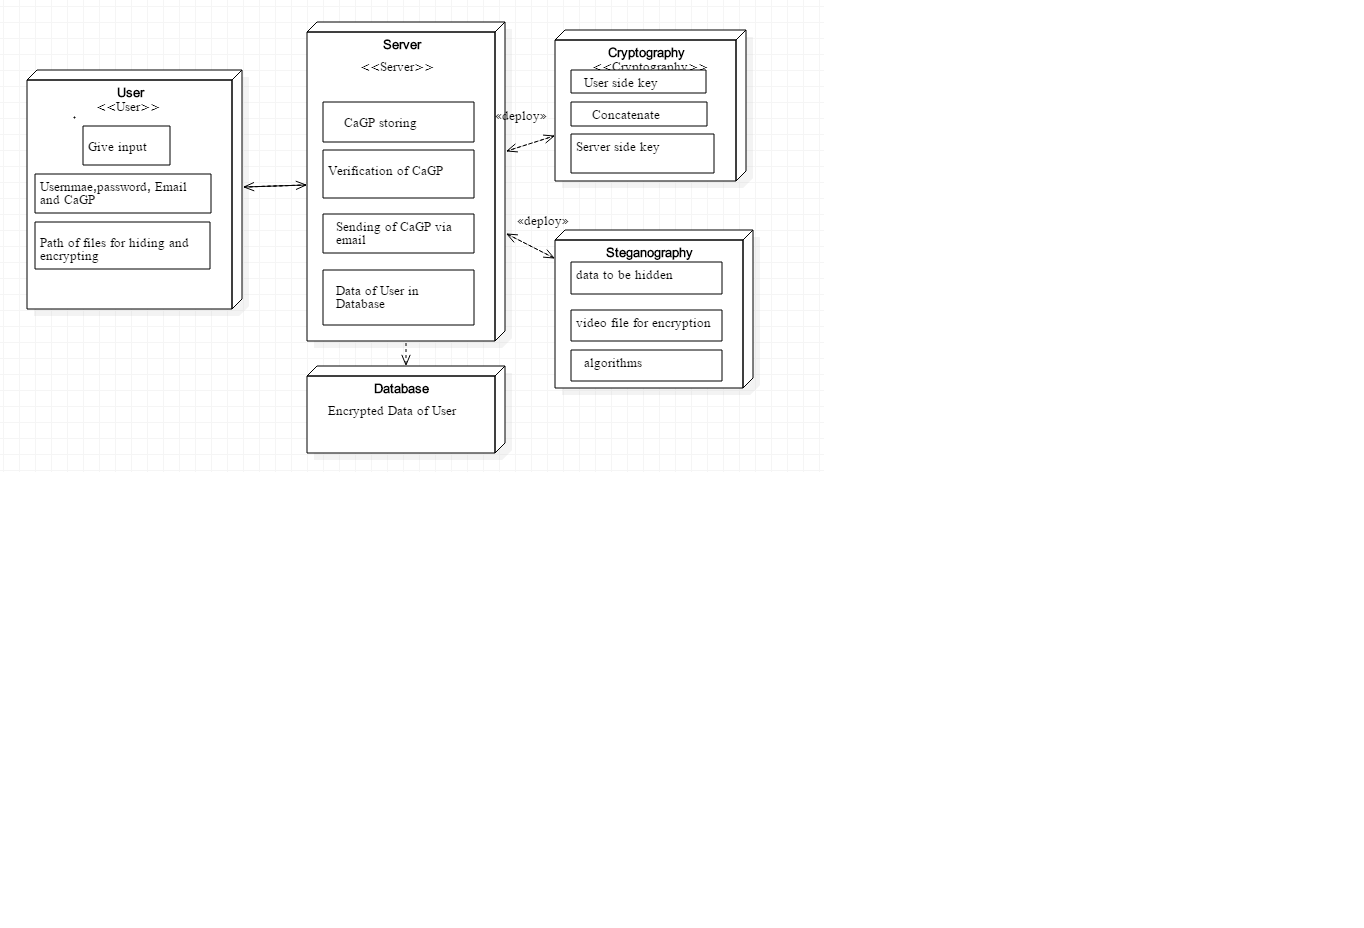
\includegraphics[scale=0.65]{deployment.png}
  \caption{Deployment Diagram}
  \end{figure}
  \pagebreak  
    \subsection*{ACTIVITY DIAGRAM}
    \begin{figure}[H]
  \centering
  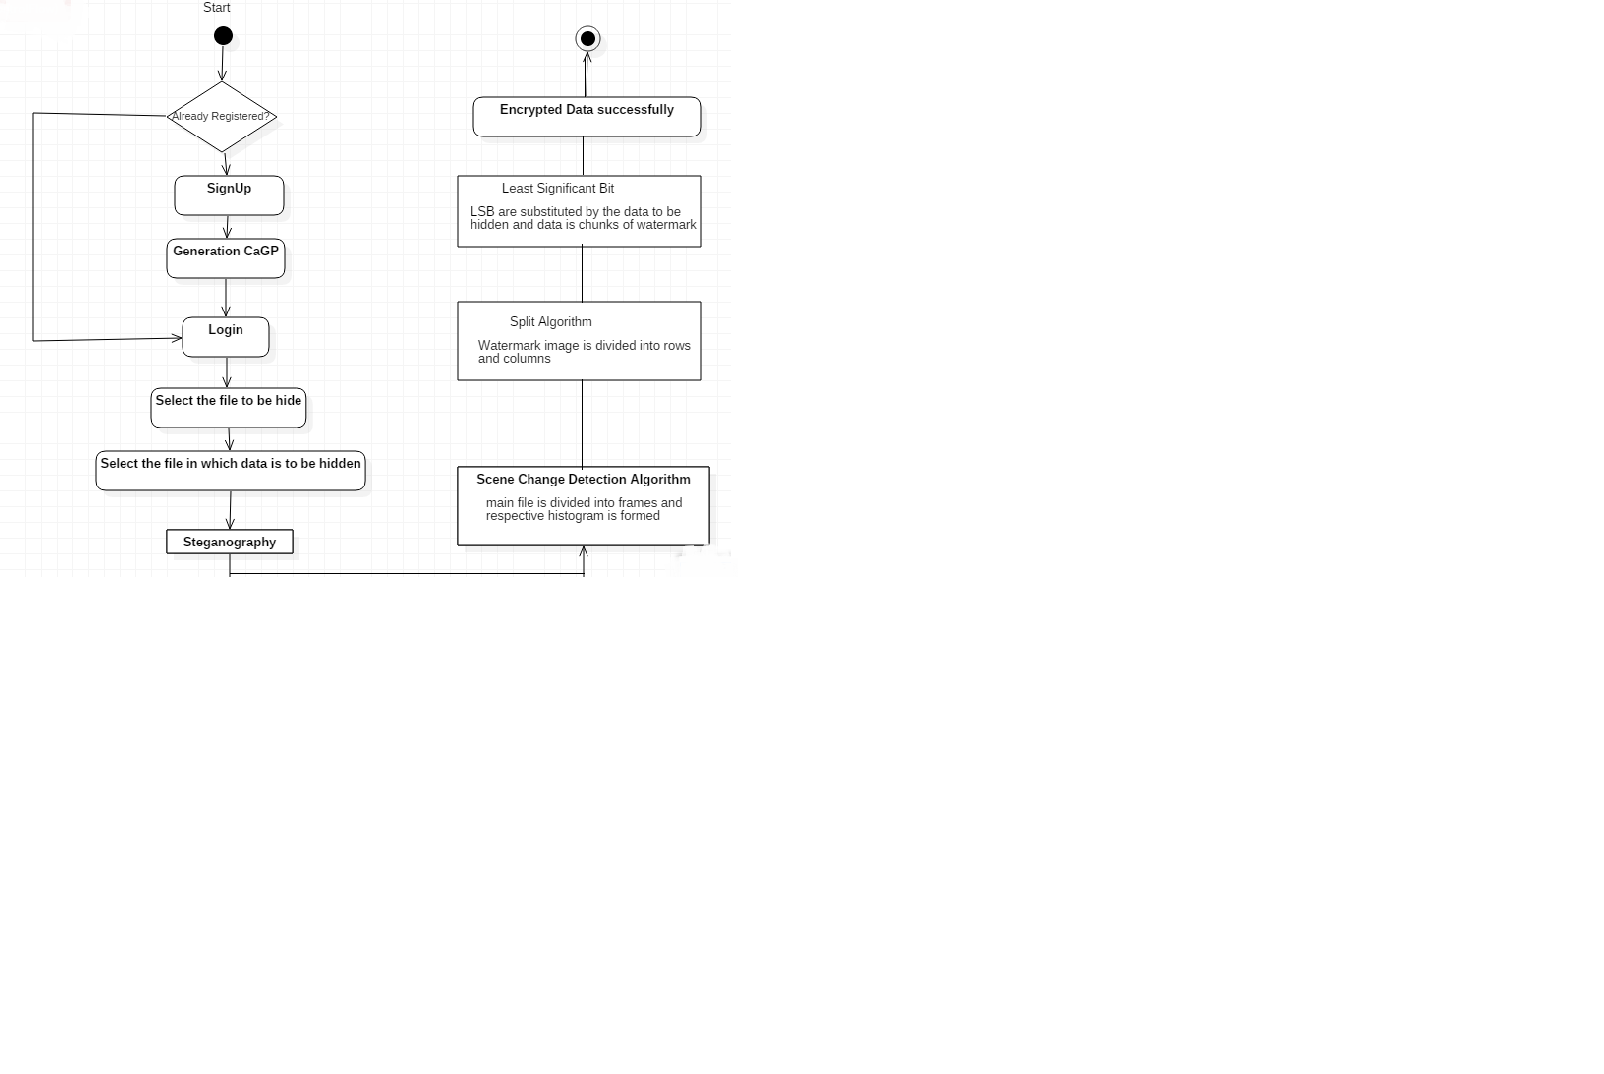
\includegraphics[scale=0.75]{activ.png}\\
  %\caption{Activity Diagram}
  
\end{figure}
    
   \pagebreak 
    \subsection*{SEQUENCE DIAGRAM}
    
    \begin{figure}[H]
  
  \centering
  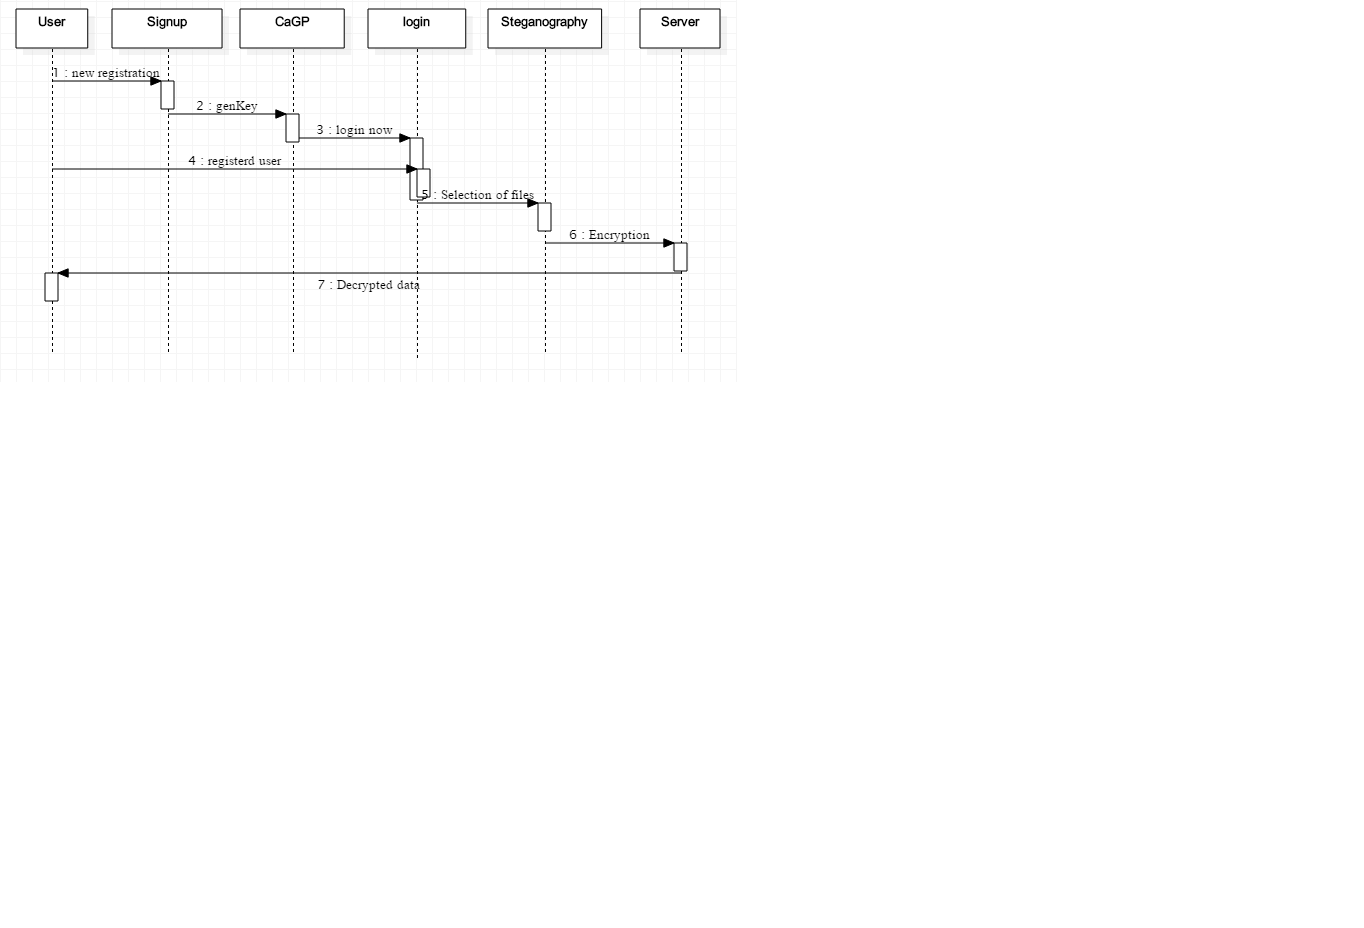
\includegraphics[scale=0.8]{sequence.png}\\
  \caption{Sequence Diagram}
  
  
\end{figure}
 \pagebreak   
    \subsection*{STATE CHART DIAGRAM}
    
    \begin{figure}[H]
  \centering
  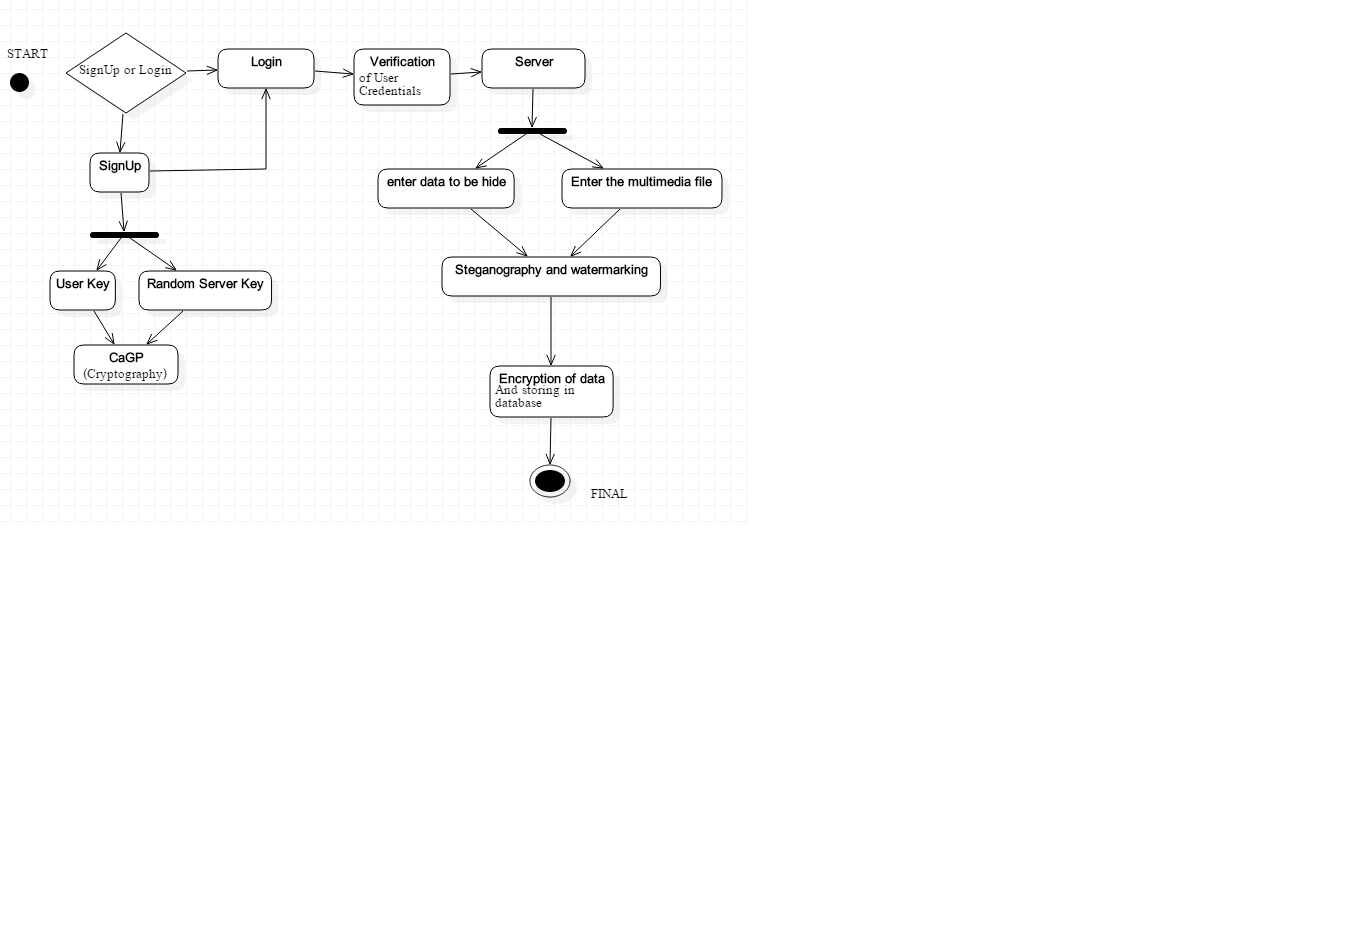
\includegraphics[scale=0.65]{State.png}\\
  \caption{State Chart Diagram}
  
\end{figure}
\pagebreak
    \subsection*{CLASS DIAGRAM}
    \begin{figure}[H]
    \centering
  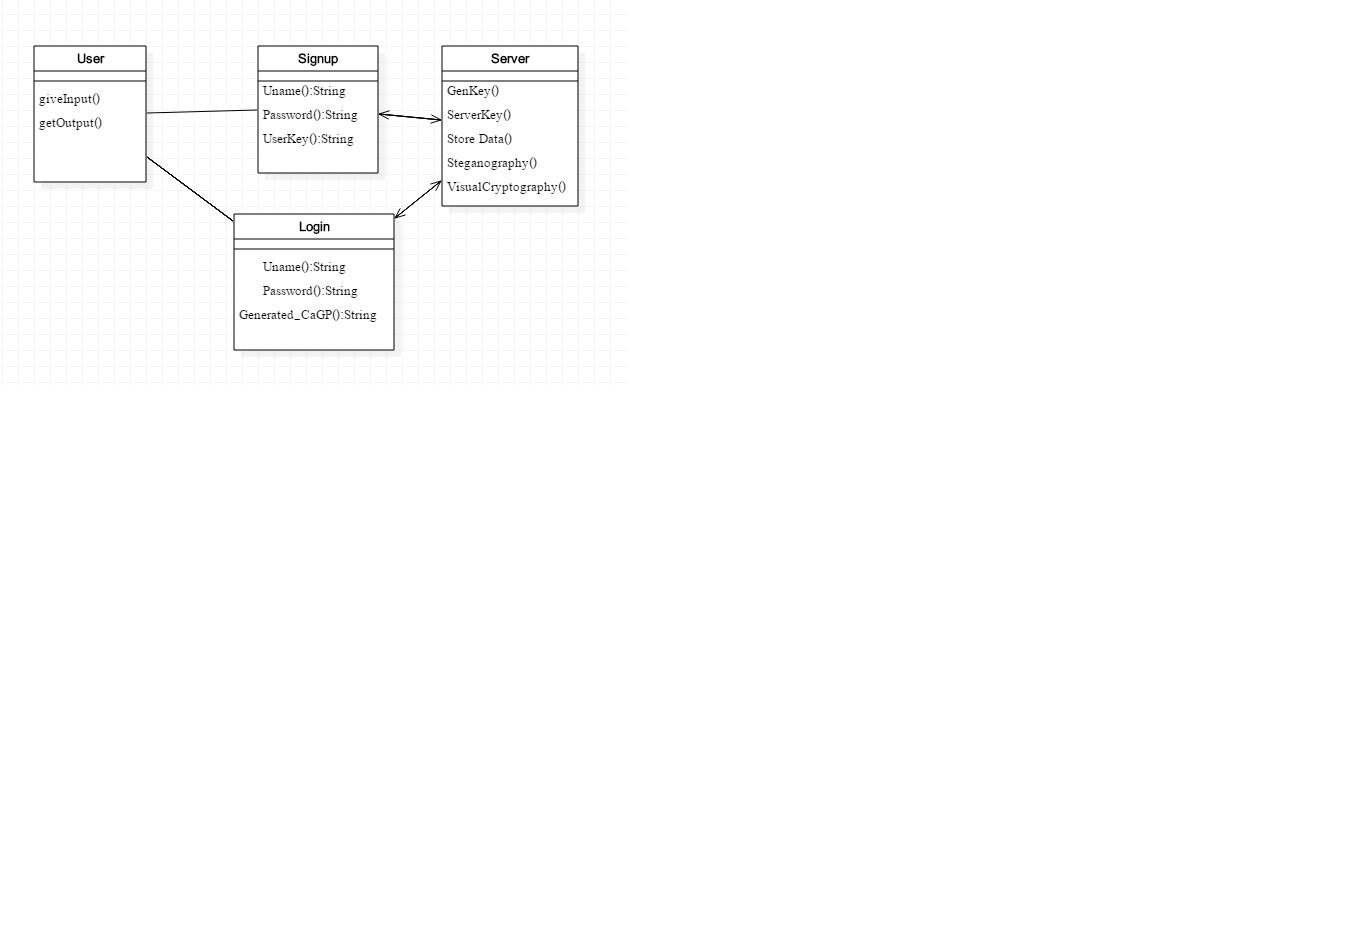
\includegraphics[scale=0.9]{Class.png}
\end{figure}


\newpage
\section*{\centering\LARGE{Lab Assignment 05}}
\subsection*{\underline{Aim}}
Testing of project problem statement using generated test data (using mathematical models, GUI, Function testing principles, if any) selection and appropriate use of testing tools, testing of UML diagram's reliability.
\noindent
\subsection*{\underline{Testing}}
\hspace{5em}Testing is a process of executing a product or application with the intention  of finding the  bugs. It can also be stated as the process of validating and verifying that a product or application meets the business and technical requirements that guided it's design and development.\\

\noindent
\begin{enumerate}
\item\textbf {Testing is about quality}
Testing is about providing a quality product to the customer.
    \begin{itemize}
    \item Quality in terms of usage.
    \item Quality in terms of look and feel.
	\item Quality in terms of data integrity.
    \item Quality in terms of security

    \end{itemize}
\item\textbf{Testing is about ideas}
Any given application can be tested in many ways. If you try out, each individual will propose a different approach and idea. We as a tester have to analyze and pick the most suitable approach.

\item\textbf{Testing is about thinking like a customer}
When we test an application, we should always think from a customer (who will use the application) point of view. Relate the flows which ideally the customer would perform on the application. Check to see if the labels/text for messages and warnings are user friendly so that the customer understands the issue if any.

\item\textbf{Testing is about coverage}
More coverage means more improved quality product. List and execute all the test combinations. Try to uncover all the odd combinations that the customer is likely to do. Prepare requirement traceability matrix. List down all the boundary conditions and negative test cases. Prioritize all the test cases.

\item\textbf{Testing is about finding defects}
Defect is described as a deviation of actual result from the requirements. This holds very true in case of testing against requirements. When checking for negative scenarios or doing ad-hoc testing we still find defects. Defects should be raised as soon as they are found and with all relevant data. People tend to miss out raising defects assuming that they are minor or just UI. Every valid defect which gets fixed adds to the quality of the product.

\item\textbf{Testing is about simplicity}
There is no point in building an application which is of high complexity and of no use. Rather we should suggest for simple design which even a lay man can use. Suggest for enhancements in the system. Users will always prefer using a system which is less complex and easy to use and understandable.

\item\textbf{Testing is about collaboration}
Testing is an activity which cannot be performed all alone.It always has to be in collaboration with the other teams like requirement, design, development, process etc.

\item\textbf{Testing is about documentation}
Documentation plays a major role in testing phase. Document the test scenarios, test cases. Prepare traceability matrix. Prepare checklist of test activities done. Prepare checklist of UI testing done. Capture all the screenshots/evidences. These documents will be very useful in future for reference in case someone has to do a round of testing again. Document all the defects in any means Microsoft Excel or defect management tool. Document the test data, environment details etc. as well.

\textbf{Testing is about time management }

Defect found later in test cycle impacts the cost and time. If we can uncover more critical defects initially in the test cycle, the more time we get to test it better. Testers always have a challenge in time management. We have to prepare the test data upfront, recreate the test data in case of failures. Track defects, test case status, check for regressions all in parallel. This makes time management really a challenge for us.


\end{enumerate}

\subsection*{\underline{Testing types}}
It describes which testing types we might follow in our testing life cycle. Here we are using:
\begin{itemize}
\item \textbf{Black Box Testing}\\
Internal system design is not considered in this type of testing. Tests are based on requirements and functionality.\\
 In our project black box testing can be used for testing:


\begin{itemize}
\item Incorrect or missing function
\item	Interface errors
\item	Errors in data structure or external job access
\item	Performance errors
\item	Initialization and termination errors.
 
\end{itemize}

In the proposed application with the help of this technique, we do not use the code to determine a test suite; rather, knowing the problem that we are trying to solve, we come up with four types of test data: 
\begin{enumerate}
\item	Easy-to-compute data,
\item	Typical data,
\item	Boundary / extreme data,
\item	Bogus data.

\end{enumerate}
But in our application we does not provide any external data, the role of user is only to give number of nodes for formation of clusters and for the formation of sink node.


\item \textbf{White Box Testing}\\
This testing is based on knowledge of the internal logic of an application’s code. Also known as Glass box Testing. Internal software and code working should be known for this type of testing. Tests are based on coverage of code statements, branches, paths, conditions.\\

In our project white box testing will be used in the implementation stage to check the android application coding and to check whether the app is connected with the database efficiently so that there is no wrong data updated in the database which the society member won’t agree with. The images should be updated automatically so that next time there is no error in validating the visitor. All this implementation should be checked in the code.




\item \textbf{Unit Testing}\\
Testing of individual software components or modules. Typically done by the programmer and not by testers, as it requires detailed knowledge of the internal program design and code. may require developing test driver modules or test harnesses.\\
In our project there are 4 modules. They are. These modules should be tested individually and the defects must be resolved before starting integration testing of these modules.


\item \textbf{System Testing}\\
Entire system is tested as per the requirements. Black-box type testing that is based on overall requirements specifications, covers all combined parts of a system.\\
   In the entire society management system as a whole, the end user requirements will be:
\begin{enumerate}
\item Maintainance of all records online.
\item Updating and choosing their activities such as casting a vote, Advertising their flat for sale, Money transaction from their accounts etc.
\item Appropriate display of vacant slots and parking of the vehicle in that slot.
\item Face detection of the visitor along with details to be stored in database and displayed on the application.
\end{enumerate}




\item \textbf{Integration Testing}\\
Testing of integrated modules to verify combined functionality after integration. Modules are typically code modules, individual applications, client and server applications on a network, etc. This type of testing is especially relevant to client/server and distributed systems. In Integration testing      will be combined and again tested and if any error in the applications on the network will be resolved.
\item \textbf{Functional Testing}
This type of testing ignores the internal parts and focus on the output is as per requirement or not. Black-box type testing geared to functional requirements of an application. The final output of our project is the proper parking of vehicles and face detection and comparison with existing images in the database.
\item \textbf{GUI Testing}

\end{itemize}

\begin{table}[ht]

\begin{tabular}{ |M{4cm}|p{5cm}|M{2.5cm}|M{3.2cm}|  }
 \hline
 \textbf{USE CASE} & \textbf{FUNCTION BEING TESTED} & \textbf{INPUT} & \textbf{EXPECTED OUTPUT}\\
 \hline
 
Data Collection & Is data collected properly? & Web data & Stored records in DB\\

\hline
 Data Classification & Is data classified into  classes as per attributes? & Data in DB & Classes of attributes\\
 
 \hline
 Pattern identification & Is unique patterns generated? & Classes from classifier & Patterns as rules.\\
 
 \hline
 Prediction & Is regions having a common pattern? & Rules from apriori & Expected output\\
  
  \hline
  
 
 \end{tabular}
 \begin{center}
 \caption{Test Cases}
 \end{center}
 \end{table}



\end{document}